% !TEX program = pdflatex
% ==============================================================================
% BIỂU MẪU BÁO CÁO VÀ BÀI TẬP KHOA CÔNG NGHỆ THÔNG TIN - ĐH KHTN (ĐHQG-HCM)
% Biên dịch bằng: PDFLaTeX
% ==============================================================================
\documentclass[12pt,a4paper]{article}
\usepackage{scrextend}
\usepackage{longtable}
\usepackage{array}
\changefontsizes{13pt}

% Nạp gói cấu hình chuẩn nhận diện FIT - HCMUS
\usepackage{fit_hcmus}

% ==============================================================================
% KHAI BÁO THÔNG TIN BÀI TẬP / ĐỒ ÁN
% ==============================================================================
\courseid{CSC14003}
\coursename{Cơ Sở Trí Tuệ Nhân Tạo}
\reportsubtitle{BÁO CÁO ĐỒ ÁN MÔN HỌC }
\title{Project 1: Bloxorz Solver}
\instructor{%
    \begin{tabular}[t]{@{}l@{}}
        TS. Bùi Tiến Lên \\
        TA. Nguyễn Thanh Tình
    \end{tabular}%
}
\classid{CQ2024/22}
\academicyear{Học kỳ I, 2026 - 2027}

% Khai báo danh sách sinh viên thực hiện
\author{
    \centering
    \begin{tabular}{c}
        Ngô Hoàng Minh - 24120381 \\
        Nguyễn Xuân Lộc - 24120369 \\
        Đỗ Ngọc Hải - 24120300 \\
        Nguyễn Thành Bảo - 24120023 \\
        Phan Nhật Minh - 24120384 \\
    \end{tabular}
}

% ==============================================================================
% CHỌN CHẾ ĐỘ HIỂN THỊ (PROJECT HOẶC ASSIGNMENT/LAB)
% Đặt true nếu là Báo cáo đồ án (có trang bìa riêng, mục lục)
% Đặt false nếu là Bài tập cá nhân / Lab ngắn gọn (dùng header đầu trang 1)
% ==============================================================================
\newif\ifisprojectreport
\isprojectreporttrue % <--- ĐỔI THÀNH \isprojectreportfalse CHO BÀI TẬP NGẮN

\begin{document}

\ifisprojectreport
    % --- CHẾ ĐỘ 1: BÁO CÁO ĐỒ ÁN MÔN HỌC (PROJECT REPORT) ---
    % Avoid reusing the first page anchor for the unnumbered cover.
    \hypersetup{pageanchor=false}
    \makecoverpage
    \hypersetup{pageanchor=true}
    
    % Trang Mục lục (chỉ hiển thị số trang La Mã ở dưới, không có header)
    \pagestyle{plain}
    \pagenumbering{roman}
    \tableofcontents
    \newpage
    % \listoffigures % Bỏ comment nếu bài viết có nhiều hình ảnh
    % \listoftables  % Bỏ comment nếu bài viết có nhiều bảng biểu
    
    % Bắt đầu nội dung chính: Bật Header chuẩn và đánh số trang Ả Rập
    \pagestyle{fancy}
    \pagenumbering{arabic}
\else
    % --- CHẾ ĐỘ 2: BÀI TẬP THỰC HÀNH / LAB NGẮN (ASSIGNMENT / LAB) ---
    \pagestyle{fancy}
    \makeassignmentheader
    \pagenumbering{arabic}
\fi

% ==============================================================================
% CÁC CHƯƠNG MỤC NỘI DUNG (SECTIONS)
% ==============================================================================
\section{Giới thiệu}
\subsection{Thông tin nhóm}
Nhóm em gồm có 05 thành viên, với thông tin và mức độ hoàn thành như sau:
\begin{table}[h!]
    \centering
    \caption{Thành viên nhóm, công việc và mức độ hoàn thành}
    \label{tab:thong_tin_nhom}
    \small
    \renewcommand{\arraystretch}{1.45}
    \setlength{\tabcolsep}{8pt}
    \setlength{\lightrulewidth}{0.25pt}
    \begin{tabularx}{\textwidth}{@{}l c >{\raggedright\arraybackslash}X >{\centering\arraybackslash}p{2.8cm}@{}}
    \toprule
    \textcolor{HCMUSBlue}{\textbf{Họ tên}} &
    \textcolor{HCMUSBlue}{\textbf{MSSV}} &
    \textcolor{HCMUSBlue}{\textbf{Công việc}} &
    \textcolor{HCMUSBlue}{\textbf{\shortstack{Mức độ\\hoàn thành}}} \\
    \midrule
    Ngô Hoàng Minh & 24120381 & & \\
    \midrule
    Nguyễn Xuân Lộc & 24120369 & & \\
    \midrule
    Đỗ Ngọc Hải & 24120300 & & \\
    \midrule
    Nguyễn Thành Bảo & 24120023 & UCS; tích hợp UI solver; benchmark và trực quan hóa & \\
    \midrule
    Phan Nhật Minh & 24120384 & & \\
    \bottomrule
    \end{tabularx}
\end{table}

\input{sections/introduction.tex}
\section{Project Planning \& Task Distribution}

\subsection{Kế hoạch triển khai dự án}

Dự án Bloxorz Solver được chia thành các nhóm công việc chính: xây dựng
logic trò chơi, phát triển giao diện, cài đặt các thuật toán tìm kiếm và
chuẩn bị báo cáo. Logic trò chơi và mô hình trạng thái là nền tảng dùng
chung, giúp các thành viên phát triển giao diện và thuật toán song song
mà vẫn sử dụng thống nhất các quy tắc di chuyển, công tắc và cầu.

Kế hoạch triển khai dưới đây được tổng hợp từ lịch sử commit trong
khoảng ngày 12/10/2026 đến 22/10/2026. Các giai đoạn có thời gian giao
nhau do nhiều mô-đun được phát triển đồng thời.

\begin{table}[H]
    \centering
    \caption{Các giai đoạn triển khai dự án}
    \label{tab:project_timeline}
    \small
    \renewcommand{\arraystretch}{1.2}
    \begin{tabularx}{\textwidth}{@{}>{\raggedright\arraybackslash}p{2.7cm}
        >{\raggedright\arraybackslash}p{2.5cm}
        >{\raggedright\arraybackslash}X@{}}
        \toprule
        \textbf{Giai đoạn} & \textbf{Thời gian} & \textbf{Nội dung chính} \\
        \midrule
        Xây dựng nền tảng & 12--15/10 &
        Khởi tạo repository và cấu trúc mã nguồn; xây dựng các đối tượng
        trò chơi, \texttt{Board}, \texttt{GameRules}, dữ liệu 20 màn chơi
        và các kiểm thử logic. \\
        \midrule
        Phát triển giao diện & 17--19/10 &
        Xây dựng ứng dụng Pygame, bộ điều khiển và hiển thị bàn chơi;
        bổ sung menu, quản lý tiến trình, hiệu ứng chuyển động và sửa
        lỗi tương tác. \\
        \midrule
        Phát triển thuật toán & 19--22/10 &
        Mô hình hóa bài toán; xây dựng khung solver dùng chung; cài đặt
        BFS, DFS, UCS và A*; bổ sung heuristic, mã đo hiệu năng và
        kiểm thử thuật toán. \\
        \midrule
        Viết báo cáo& Từ ngày 19 &
        Viết báo cáo LaTeX, chuẩn bị video\\
        \bottomrule
    \end{tabularx}
\end{table}

\subsection{Phân công nhiệm vụ}

\begin{table}[H]
    \centering
    \caption{Phân công nhiệm vụ của các thành viên}
    \label{tab:task_distribution}
    \small
    \renewcommand{\arraystretch}{1.2}
    \begin{tabularx}{\textwidth}{@{}>{\raggedright\arraybackslash}p{3.5cm}
        >{\raggedright\arraybackslash}X@{}}
        \toprule
        \textbf{Thành viên} & \textbf{Nhiệm vụ} \\
        \midrule
        Ngô Hoàng Minh &
        \textbullet\ Khởi tạo dự án, tổ chức mã nguồn và dữ liệu dùng chung. \newline
        \textbullet\ Xây dựng \texttt{Board}, \texttt{GameRules}, bộ 20 màn chơi và công cụ trực quan hóa bản đồ. \newline
        \textbullet\ Mô hình hóa bài toán, xây dựng khung solver, cài đặt A* và heuristic. \newline
        \textbullet\ Viết kiểm thử logic, bản đồ và A*; sửa lỗi GUI. \newline \\
        \midrule
        Phan Nhật Minh &
        \textbullet\ Định nghĩa các loại ô và cầu; khai báo thư viện phụ thuộc. \newline
        \textbullet\ Cài đặt thuật toán BFS. \newline
        \textbullet\ Bổ sung mã đo thời gian, bộ nhớ, số nút mở rộng và độ dài lời giải. \\
        \midrule
        Nguyễn Thành Bảo &
        \textbullet\ Xây dựng cơ chế khối, công tắc và tương tác với cầu. \newline
        \textbullet\ Tích hợp các thành phần vào API backend dùng chung. \newline
        \textbullet\ Cài đặt UCS, viết kiểm thử và tài liệu thuật toán. \\
        \midrule
        Đỗ Ngọc Hải &
        \textbullet\ Xây dựng ứng dụng Pygame, bộ điều khiển và hiển thị trò chơi. \newline
        \textbullet\ Quản lý tiến trình, sửa hiệu ứng rơi và viết kiểm thử giao diện, chuyển động. \newline
        \textbullet\ Cài đặt DFS, bổ sung cấu trúc kết quả tìm kiếm và kiểm thử DFS. \\
        \midrule
        Nguyễn Xuân Lộc &
        \textbullet\ Điều chỉnh tỷ lệ hiển thị bàn chơi, khối và ký hiệu công tắc. \newline
        \textbullet\ Hoàn thiện menu, màn hình chiến thắng và hiệu ứng ngôi sao. \newline
        \textbullet\ Cải thiện hiệu ứng rơi và bổ sung cơ chế tự khởi động lại màn chơi khi thua. \\
        \bottomrule
    \end{tabularx}
\end{table}


\section{Thiết kế BackEnd}
\subsection{Tổ chức và mô hình trạng thái}

BackEnd được tổ thiết kế thành 3 thành phần: các đối tượng trong \path{BackEnd/objects}, bộ luật trong game
\path{BackEnd/logic}, các thuật toán tìm kiếm trong \path{BackEnd/Solver}. Giao diện và các solver sử dụng chung bộ luật
để đảm bảo tính nhất quán.

Lớp \texttt{Board} quản lí các ô, công tắc và trạng thái hiện tại. Trạng thái tìm kiếm được biểu diễn bởi
\[
s=(P,o,a,B)
\]
trong đó $P$ là các tọa độ khối chiếm giữ, $o$ là hướng đặt hoặc trạng thái tách, $a$ là khối con đang điều khiển và $B$ là tập cầu đang mở.

\texttt{BlockState} lưu $P$, $o$, $a$; \texttt{GameState} kết hợp
\texttt{BlockState} với $B$. Hai lớp được khai báo bất biến, cho phép
dùng trực tiếp làm khóa trong \texttt{visited} hoặc bảng chi phí.
Tọa độ sử dụng dạng $(x,y)$, với $x$ tăng sang phải và $y$ tăng xuống dưới.

\subsection{Thiết kế hướng đối tượng}

Lớp \texttt{Tile} là lớp cơ sở của các loại ô. Các lớp con định nghĩa khả năng đỡ khối thông qua \texttt{can\_support()}:

\begin{itemize}
    \item \texttt{FloorTile}, \texttt{Goal}: cho phép khối nằm trên ô;
    điều kiện chiến thắng được kiểm tra riêng.
    \item \texttt{EmptyCell}: không đỡ khối. Vị trí không có đối tượng
    ô trên bàn cũng được xem là khoảng trống.
    \item \texttt{FragileTile}: không đỡ khối nguyên vẹn đang đứng;
    cho phép khối nằm hoặc khối con sau khi tách.
    \item \texttt{Bridge}: chỉ đỡ khối khi ID cầu thuộc tập
    \texttt{open\_bridges} của trạng thái hiện tại.
\end{itemize}

Lớp \texttt{Switch} kế thừa \texttt{Tile}. \texttt{SoftSwitch} kích hoạt
khi có phần khối đè lên; \texttt{HeavySwitch} và \texttt{SplitSwitch}
chỉ kích hoạt khi khối nguyên vẹn đứng trên công tắc.
Các liên kết \texttt{SwitchBridgeLink} xác định cầu bị tác động theo
chế độ đảo trạng thái (\texttt{TOGGLE}) hoặc đặt trạng thái
(\texttt{SET}). \texttt{SplitSwitch} còn lưu hai vị trí dịch chuyển
của các khối con.

\begin{figure}[htbp]
    \centering
    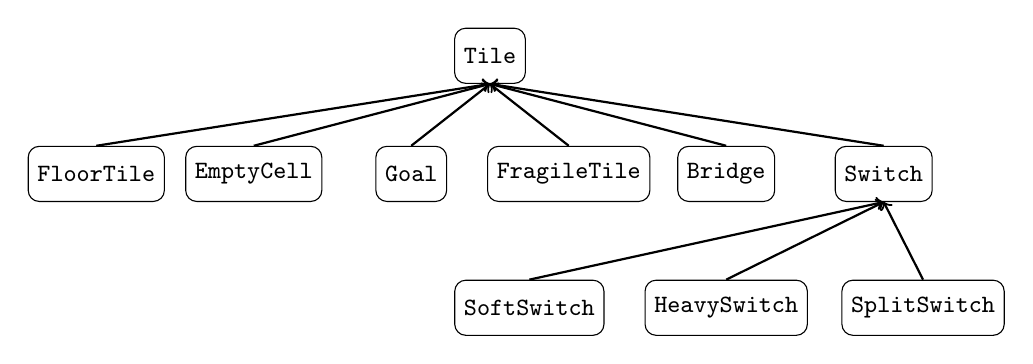
\begin{tikzpicture}[
        box/.style={
            draw, rounded corners,
            minimum height=0.7cm,
            align=center, font=\small
        },
        edge/.style={->, thick}
    ]
        \node[box] (tile) at (0,0) {\texttt{Tile}};

        \node[box] (floor) at (-5,-1.5) {\texttt{FloorTile}};
        \node[box] (empty) at (-3,-1.5) {\texttt{EmptyCell}};
        \node[box] (goal) at (-1,-1.5) {\texttt{Goal}};
        \node[box] (fragile) at (1,-1.5) {\texttt{FragileTile}};
        \node[box] (bridge) at (3,-1.5) {\texttt{Bridge}};
        \node[box] (switch) at (5,-1.5) {\texttt{Switch}};

        \foreach \child in {floor,empty,goal,fragile,bridge,switch}
            \draw[edge] (\child.north) -- (tile.south);

        \node[box] (soft) at (0.5,-3.2) {\texttt{SoftSwitch}};
        \node[box] (heavy) at (3,-3.2) {\texttt{HeavySwitch}};
        \node[box] (split) at (5.5,-3.2) {\texttt{SplitSwitch}};

        \foreach \child in {soft,heavy,split}
            \draw[edge] (\child.north) -- (switch.south);
    \end{tikzpicture}
    \caption{Quan hệ kế thừa giữa các loại ô.
    Mũi tên hướng từ lớp con đến lớp cha.}
    \label{fig:tile_classes}
\end{figure}

\begin{figure}[htbp]
    \centering
    \begin{tikzpicture}[
        box/.style={
            draw, rounded corners,
            minimum width=2.6cm, minimum height=0.8cm,
            align=center, font=\small
        },
        edge/.style={->, thick},
        note/.style={font=\scriptsize, fill=white, inner sep=2pt}
    ]
        \node[box] (solver) at (0,0) {\texttt{BaseSolver}};
        \node[box] (rules) at (4,0) {\texttt{GameRules}};
        \node[box] (board) at (8,0) {\texttt{Board}};
        \node[box] (state) at (8,-1.8) {\texttt{GameState}};
        \node[box] (block) at (4,-1.8) {\texttt{BlockState}};
        \node[box] (tiles) at (8,-3.6) {Các đối tượng \texttt{Tile}};

        \draw[edge] (solver) -- node[note,above]{sử dụng} (rules);
        \draw[edge] (rules) -- node[note,above]{tham chiếu} (board);
        \draw[edge] (board) -- node[note,right]{trạng thái hiện tại} (state);
        \draw[edge] (state) -- node[note,above]{chứa} (block);
        \draw[edge] (board.east) -- ++(1.4,0)
            |- node[note,pos=0.75,right]{quản lý} (tiles.east);
    \end{tikzpicture}
    \caption{Quan hệ sử dụng và chứa giữa các lớp chính,
    không biểu diễn quan hệ kế thừa.}
    \label{fig:backend_relations}
\end{figure}

Các lớp \texttt{BFSSolver}, \texttt{DFSSolver}, \texttt{UCSSolver}
và \texttt{AStarSolver} kế thừa \texttt{BaseSolver}, dùng chung
cách sinh trạng thái và truy vết lời giải.

\subsection{Các hàm cơ sở}
\begin{description}
    \item[\texttt{init\_map(map\_name)}]
    Đọc dữ liệu JSON, tạo các đối tượng trên bàn và khởi tạo
    trạng thái bắt đầu.

    \item[\texttt{Board.initialize\_game\_state()}]
    Khởi tạo trạng thái khối và tập cầu mở theo cấu hình
    \texttt{initial\_open}.

    \item[\texttt{Board.get\_tile(position)}]
    Tra cứu ô tại tọa độ, ưu tiên cầu phủ lên ô nền;
    trả \texttt{None} nếu không có ô.

    \item[\texttt{Board.add\_game\_state(state)}]
    Cập nhật trạng thái hiện tại và đồng bộ thuộc tính khối
    của bàn chơi.

    \item[\texttt{GameRules.is\_valid(state)}]
    Kiểm tra hình dạng khối, cấu hình cầu và khả năng đỡ khối
    tại mọi vị trí đang chiếm giữ.

    \item[\texttt{GameRules.apply\_action(state, action)}]
    Tính trạng thái kế tiếp sau một hành động. Hàm xử lý di chuyển,
    công tắc, cầu và tách/ghép khối; trả \texttt{None} nếu không hợp lệ,
    không sửa bàn chơi hay trạng thái đầu vào.

    \item[\texttt{GameRules.is\_goal(state)}]
    Kiểm tra trạng thái hợp lệ và khối nguyên vẹn đứng thẳng
    trên ô đích.

    \item[\texttt{BaseSolver.successors(state)}]
    Sinh các bộ $(action,next\_state,cost)$ hợp lệ theo thứ tự
    hành động chung, với chi phí mỗi hành động bằng 1.

    \item[\texttt{BaseSolver.reconstruct\_path(goal\_node)}]
    Lần theo \texttt{parent}, thu thập \texttt{action} và đảo
    thứ tự để trả chuỗi hành động từ đầu đến đích.
\end{description}

\subsection{Luồng xử lý hành động}
Với hành động di chuyển, \texttt{apply\_action()} tính tư thế và vị trí mới, kiểm tra khả năng đứng trên các ô, áp dụng công tắc rồi kiểm
tra lại trạng thái sau khi hành động. Nếu khối đang tách, hai khối con sẽ được hợp nhất khi nằm kề nhau. Hành động \texttt{Switch} chỉ đổi
khối đang điều khiển và chỉ hợp lệ khi khối đang được tách.

Giao diện cập nhật bàn chơi bằng trạng thái trả về, các solver dùng trạng thái đó để mở rộng tìm kiếm. Do đó chơi thủ công và phát lại lời
giải đều tuân theo cùng một bộ luật.

\section{Thiết kế FrontEnd}
\label{sec:frontend}

\subsection{Tổ chức module và luồng dữ liệu}

FrontEnd được xây dựng bằng \textit{Pygame}, tách thành các module theo
vai trò riêng biệt trong \path{FrontEnd/}:
\begin{itemize}
    \item \texttt{app.py} - lớp \texttt{App}, điều phối toàn bộ vòng lặp
    giao diện: xử lý sự kiện, vẽ khung hình, chuyển chế độ chơi và quản lý
    tiến trình tìm kiếm.
    \item \texttt{controller.py} - lớp \texttt{GameController}, cầu nối 
    giữa giao diện và \texttt{BackEnd}.
    \item \texttt{renderer.py} - dựng hình bàn chơi theo phép chiếu
    isometric.
    \item \texttt{wood.py} - dựng hình khối gỗ 3D và hoạt ảnh lăn/rơi.
    \item \texttt{fall\_motion.py} - tính tư thế rơi của khối khi thua.
    \item \texttt{progress.py} - lưu tiến trình chơi, tính sao và điều
    kiện mở khóa màn.
\end{itemize}

\begin{figure}[htbp]
    \centering
    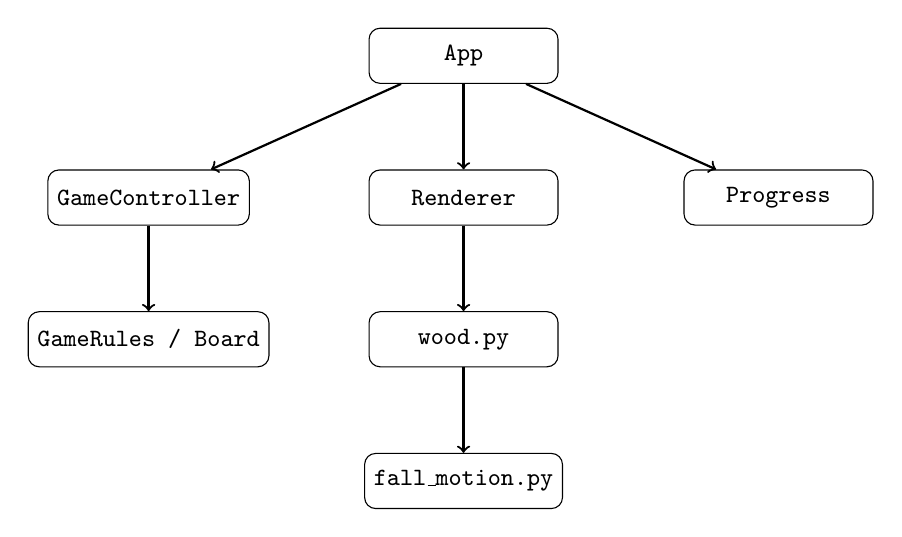
\begin{tikzpicture}[
        box/.style={draw, rounded corners, minimum height=0.7cm,
                    minimum width=2.4cm, align=center, font=\small},
        edge/.style={->, thick}
    ]
        \node[box] (app) at (0,0) {\texttt{App}};
        \node[box] (controller) at (-4,-1.8) {\texttt{GameController}};
        \node[box] (renderer) at (0,-1.8) {\texttt{Renderer}};
        \node[box] (progress) at (4,-1.8) {\texttt{Progress}};
        \node[box] (rules) at (-4,-3.6) {\texttt{GameRules / Board}};
        \node[box] (wood) at (0,-3.6) {\texttt{wood.py}};
        \node[box] (fall) at (0,-5.4) {\texttt{fall\_motion.py}};

        \draw[edge] (app) -- (controller);
        \draw[edge] (app) -- (renderer);
        \draw[edge] (app) -- (progress);
        \draw[edge] (controller) -- (rules);
        \draw[edge] (renderer) -- (wood);
        \draw[edge] (wood) -- (fall);
    \end{tikzpicture}
    \caption{Quan hệ sử dụng giữa các module của FrontEnd.}
    \label{fig:frontend_modules}
\end{figure}

Dữ liệu đi theo một chiều: \texttt{BackEnd} sinh \texttt{GameState} mới
sau mỗi hành động, \texttt{GameController} lưu lại trạng thái đó, còn
\texttt{Renderer}/\texttt{wood.py} chỉ đọc trạng thái và tham số hoạt ảnh
để vẽ, không module FrontEnd nào chỉnh sửa trực tiếp \texttt{Board} hay
\texttt{GameRules} ngoài thông qua \texttt{GameController}. Nhờ vậy chơi
thủ công, hiển thị lại lời giải và vẽ lại khung hình khi đổi kích thước cửa
sổ đều dùng chung một nguồn trạng thái duy nhất.

\subsection{Thiết kế các lớp chính}

Các lớp của FrontEnd được tổ chức theo quan hệ
\textit{composition}: mỗi lớp chỉ giữ tham chiếu tới đối tượng cần dùng
chứ không sao chép trạng thái, tránh lệch dữ liệu giữa giao diện và bộ
luật.
\begin{itemize}
    \item \texttt{GameController} đóng gói một \texttt{Board} và \texttt{GameRules}
    cho một màn chơi, đồng thời lưu \texttt{history} (các cặp trạng thái-hành
    động đã thực hiện) phục vụ hiển thị số bước và chơi lại màn.
    \item Hàm \texttt{move(action)} gọi \texttt{GameRules.apply\_action()}; nếu kết quả
    là \texttt{None} thì trạng thái được đánh dấu \texttt{"lost"}, ngược lại
    trạng thái mới được ghi vào \texttt{Board} và kiểm tra đích bằng
    \texttt{GameRules.is\_goal()}. Vì chơi thủ công và phát lại lời giải đều
    đi qua cùng hàm này, hành vi luôn khớp với bộ luật dùng trong tìm kiếm.
    \item Tham số \texttt{replay} phân biệt hai luồng gọi: khi \texttt{replay=False}
    (người chơi tự di chuyển), lời giải và kết quả benchmark cũ bị xóa qua
    \texttt{clear\_solution()} vì chúng không còn khớp với trạng thái hiện tại;
    khi \texttt{replay=True}, lịch sử tìm kiếm được giữ nguyên.
    \item Các hàm \texttt{set\_solution()}, \texttt{start\_replay()} và
    \texttt{step()} phục vụ riêng cho luồng phát lại lời giải, được mô tả
    chi tiết ở Mục~\ref{sec:ui_solver}.
    \item \texttt{Renderer} không giữ trạng thái trò chơi: mọi lời gọi vẽ nhận
    \texttt{state} và tham số hoạt ảnh làm đầu vào, nên cùng một lớp có thể vẽ
    cả khi chơi thủ công, khi phát lại và khi chỉ xem lại một khung hình tĩnh.
    \item \texttt{Progress} tách biệt hoàn toàn khỏi logic trò chơi, chỉ nhận
    tên màn và số bước để tính sao và lưu tiến độ xuống đĩa, nên không phụ thuộc
    \texttt{GameRules} và không bị ảnh hưởng nếu luật chơi thay đổi.
\end{itemize}

\subsection{Các cơ chế dựng hình và hoạt ảnh}
\label{sec:frontend_render}

\begin{description}
    \item[Phép chiếu isometric] \texttt{Renderer.board()} chiếu tọa độ
    lưới $(x,y,z)$ sang tọa độ màn hình bằng
    \[
        (u,v) = \big(o_x + (x-y)\cdot s,\; o_y + (x+y)\cdot s/2 - z\cdot s\big),
    \]
    với tỉ lệ $s$ tính để bàn chơi luôn vừa khung hiển thị và gốc chiếu
    $(o_x,o_y)$ đặt tại tâm khung.

    \item[Vẽ ô (\texttt{prism()})] Mỗi ô được vẽ bằng một hình hộp thấp,
    tô màu theo loại ô: nền, ô dễ vỡ (cam), cầu (nâu, gạch chéo đỏ khi
    đóng) và công tắc (vòng tròn \texttt{O}/\texttt{X}/hai chấm tương ứng
    \texttt{SoftSwitch}/\texttt{HeavySwitch}/\texttt{SplitSwitch}). Cầu
    đang đóng được bỏ qua khi vẽ nhưng vẫn vẽ ô nền dưới cầu, vì
    \texttt{Board} cho phép cầu phủ lên một ô khác; trạng thái cầu dùng
    để vẽ là trạng thái \textit{trước} khi hoạt ảnh lăn bắt đầu, để cầu
    không đổi trạng thái giữa lúc khối đang lăn qua.

    \item[Hoạt ảnh lăn (\texttt{wood.py})] Khối xoay quanh cạnh tiếp đất
    theo hướng di chuyển (tham số \texttt{pivot}), với góc xoay
    $\theta(t) = \mathrm{smoothstep}(t)\cdot\pi/2$, $t\in[0,1]$ theo thời
    gian lăn (tối đa 0.28s hoặc theo tốc độ phát lại), trong đó
    \textit{smoothstep} là $t^2(3-2t)$. Khi thắng, khối hạ thấp dần và
    các mặt bị cắt tại $z=0$ (\texttt{clip\_floor}) để không hiển thị
    phần khối chìm dưới sàn.

    \item[Hoạt ảnh rơi (\texttt{fall\_motion.py})] \texttt{GameRules} chỉ
    trả \texttt{None} cho hành động khiến khối rơi, không giữ lại trạng
    thái trung gian để vẽ. \texttt{prepare\_fall()} tính lại cục bộ, chỉ
    phục vụ hiển thị: áp dụng phần xoay của hành động
    (\texttt{rules.\_roll()}) để suy ra vị trí "định đáp", xác định vị
    trí còn được đỡ (\texttt{supported}) và ô dễ vỡ bị vỡ
    (\texttt{broken}); nếu còn đúng một điểm tựa, cạnh lật được xác định
    làm trục xoay. \texttt{fall\_vertex()} dựng chuyển động hai giai
    đoạn: lật quanh cạnh đỡ trong $0.36$s đầu, sau đó rơi tự do với gia
    tốc không đổi ($z \mathrel{-}= 2.5t + 15t^2$), khối mờ dần ở cuối
    hoạt ảnh.

    \item[Hoạt ảnh sao (\texttt{draw\_victory()})] Độc lập với khối 3D:
    ba ngôi sao bật ra lệch nhau $0.12$s mỗi sao, phóng to theo hàm
    \textit{ease-out-back}
    \[
        f(t) = 1 + c_3(t-1)^3 + c_1(t-1)^2, \qquad c_1 = 1.70158,\ c_3 = c_1+1,
    \]
    tạo hiệu ứng vượt quá kích thước đích rồi co lại, khác với
    \textit{smoothstep} êm dùng cho khối gỗ. Số sao đạt được tô vàng, số
    còn lại tô xám.
\end{description}

\subsection{Luồng xử lý và tiến trình chơi}

Vòng lặp chính trong \texttt{App.run()} lần lượt: xử lý sự kiện bàn
phím/chuột, cập nhật tiến trình tìm kiếm đang chạy nếu có, tự động phát bước kế tiếp khi đang ở chế độ
\textit{Replay}, rồi vẽ lại khung hình. Phím mũi tên/WASD ứng với bốn
hướng lăn trên bàn isometric (không trùng trục màn hình do góc chiếu),
\texttt{Space} đổi khối con khi đã tách, \texttt{R} khởi động lại màn,
\texttt{Esc} hủy tìm kiếm hoặc đóng panel đang mở theo thứ tự ưu tiên. Mỗi
di chuyển hợp lệ hoặc không hợp lệ đều tạo một bản ghi \texttt{animation}
dùng chung bởi \texttt{Renderer} và \texttt{wood.py} để phát đúng hoạt ảnh
tương ứng.

Khi \texttt{GameController} báo trạng thái \texttt{"won"} ở chế độ chơi
thủ công,  \texttt{App.check\_victory()} đợi hoạt ảnh kết thúc rồi gọi
\texttt{Progress.complete(map\_name, moves)}: số sao được tính bằng
\texttt{stars\_for()} so với số bước mục tiêu (\texttt{TARGETS}), bản ghi
tốt nhất được giữ lại và ghi xuống \path{.save/progress.json} theo mẫu
ghi-tạm-rồi-đổi-tên (\texttt{.tmp} rồi \texttt{replace()}) để tránh hỏng
file nếu chương trình bị tắt giữa lúc ghi. \texttt{unlocked(level)} yêu
cầu mọi màn có số thứ tự nhỏ hơn đã hoàn thành, tức mở khóa tuần tự theo
chiến dịch. Khi trạng thái \texttt{"lost"}, \texttt{App.check\_defeat()}
tự khởi động lại màn sau khi hoạt ảnh rơi phát xong, không cần người chơi
nhấn \texttt{R}.

Chế độ \textit{Solve by algorithm} dùng lại đúng \texttt{GameController}
và \texttt{Renderer} nói trên nhưng không gọi \texttt{check\_victory()}/
\texttt{Progress.complete()} trong lúc phát lại, để kết quả giải bằng
thuật toán không ghi sao hay mở khóa chiến dịch thay người chơi.


\section{Tìm kiếm theo chiều rộng (BFS)}

\subsection{Cấu trúc dữ liệu và quá trình tìm kiếm}
Thuật toán Tìm kiếm theo chiều rộng (Breadth-First Search - BFS) duyệt qua không gian trạng thái bằng cách mở rộng tất cả các nút ở độ sâu hiện tại trước khi chuyển sang các nút ở độ sâu lớn hơn. 

Trong đồ án này, thuật toán BFS được cài đặt kế thừa từ lớp \texttt{BaseSolver}, với các cấu trúc dữ liệu cốt lõi như sau:
\begin{itemize}
    \item \textbf{Cấu trúc Hàng đợi (Queue):} Sử dụng cấu trúc dữ liệu \texttt{deque} từ thư viện \texttt{collections} của Python. Việc sử dụng \texttt{deque} giúp tối ưu hóa thời gian thao tác thêm và lấy phần tử ở hai đầu với độ phức tạp $O(1)$, khắc phục được hiện tượng nghẽn cổ chai của \texttt{list} thông thường khi xử lý số lượng nút lớn.
    \item \textbf{Quản lý trạng thái đã duyệt (Visited Set):} Sử dụng một \texttt{set} để lưu trữ các trạng thái (\texttt{GameState}) đã được mở rộng. Cơ chế này đóng vai trò quan trọng trong việc phát hiện chu trình (cycle detection), đảm bảo thuật toán không bị rơi vào vòng lặp vô tận khi khối hộp di chuyển qua lại giữa các ô đã đi qua.
    \item \textbf{Lưu vết đường đi (SearchNode):} Mỗi trạng thái được bọc trong một đối tượng \texttt{SearchNode}, lưu trữ tham chiếu \texttt{parent} trỏ về nút cha và hành động (\texttt{action}) đã thực hiện. Khi chạm đến ô đích, bộ giải truy vết ngược từ nút đích về nút gốc để tạo thành chuỗi lời giải hoàn chỉnh đưa vào giao diện.
\end{itemize}

\subsection{Tính chất và đánh giá}
\begin{itemize}
    \item \textbf{Tính đầy đủ (Completeness):} BFS đảm bảo tính đầy đủ. Do không gian trạng thái của trò chơi Bloxorz là một đồ thị hữu hạn (giới hạn bởi kích thước bản đồ và các hướng nằm của khối), BFS chắc chắn sẽ tìm thấy lời giải nếu màn chơi đó thực sự có đường đi đến đích.
    \item \textbf{Tính tối ưu (Optimality):} Trong bài toán Bloxorz, mỗi bước di chuyển (trượt, lăn, lật khối) đều có chi phí bước đi là $1$. Vì chi phí bước đi là đồng nhất, giải pháp do BFS tìm ra luôn là giải pháp tối ưu về số lượng hành động (đường đi ngắn nhất).
    \item \textbf{Độ phức tạp bộ nhớ (Space Complexity):} Nhược điểm lớn nhất của BFS là tiêu tốn quá nhiều dung lượng bộ nhớ (Peak Memory). Trong trường hợp xấu nhất, nó phải lưu trữ toàn bộ biên (frontier) của đồ thị tìm kiếm, dẫn đến độ phức tạp không gian là $O(b^d)$ (với $b$ là hệ số phân nhánh trung bình, $d$ là độ sâu của lời giải). Điều này thể hiện rõ trong các biểu đồ Benchmark khi đo lường RAM tiêu thụ trên các bản đồ cấp độ khó.
\end{itemize}

\begin{algorithm}[H]
\caption{Thuật toán BFS}
\label{alg:bfs}
\begin{algorithmic}[1]
\Require Trạng thái đầu $s_0$, bộ luật sinh trạng thái kế tiếp
\Ensure Chuỗi hành động hợp lệ hoặc không có lời giải
\State $Q \gets$ hàng đợi (queue) chứa node gốc của $s_0$
\State $visited \gets \{s_0\}$
\While{$Q$ chưa rỗng}
    \State Lấy node $n$ khỏi đầu $Q$
    \If{$state(n)$ là đích}
        \State \Return chuỗi hành động truy vết từ $n$
    \EndIf
    \State $children \gets$ các successor hợp lệ của $state(n)$
    \For{mỗi $(a,s',c)$ trong $children$}
        \If{$s' \notin visited$}
            \State Thêm $s'$ vào $visited$
            \State Tạo node con với trạng thái $s'$, cha $n$, hành động $a$
            \State Gán độ sâu $depth(n)+1$ và chi phí $g(n)+c$
            \State Đưa node con vào cuối $Q$
        \EndIf
    \EndFor
\EndWhile
\State \Return không có lời giải
\end{algorithmic}
\end{algorithm}
\subsection{Tìm kiếm theo chiều sâu (DFS)}

\subsubsection{Mô hình trạng thái và chi phí}
DFS tìm một chuỗi hành động hợp lệ đưa khối gỗ đến đích bằng cách ưu tiên duyệt theo chiều sâu. Mỗi trạng thái là một \texttt{GameState} gồm vị trí,
hướng khối, khối gỗ đang điều khiển và tập cầu đang mở.

Các hành động gồm \texttt{UP}, \texttt{DOWN}, \texttt{LEFT},
\texttt{RIGHT} và \texttt{SWITCH}. Trạng thái kế tiếp được sinh bằng
\texttt{GameRules.apply\_action()}, bảo đảm xử lý thống nhất ô dễ vỡ,
công tắc, cầu và tách/ghép khối. Mọi hành động có chi phí bằng 1,
kể cả đổi khối con. Với đường đi gồm $k$ hành động:
\[
    g(n)=\sum_{i=1}^{k}c_i=k.
\]
DFS lưu chi phí đường đi nhưng không dùng chi phí để chọn node mở rộng. Vì vậy thuật toán DFS không đảm bảo tìm được đường đi tối ưu nhất.

\subsubsection{Cấu trúc dữ liệu và quá trình tìm kiếm}
Lớp \texttt{DFSSolver} kế thừa \texttt{BaseSolver}, sử dụng ngăn xếp LIFO và tập \texttt{visited} chứa toàn bộ \texttt{GameState} 
để chống lặp. Trạng thái được đánh dấu khi node được lấy khỏi ngăn xếp, node có trạng thái đã được thăm sẽ được bỏ qua.

Các node con được thêm theo thứ tự ngược để ưu tiên xử lý
\texttt{UP} $\rightarrow$ \texttt{DOWN} $\rightarrow$ \texttt{LEFT}
$\rightarrow$ \texttt{RIGHT} $\rightarrow$ \texttt{SWITCH}.
Khi gặp đích, thuật toán truy vết các trường \texttt{parent} và
\texttt{action} của \texttt{SearchNode} để trả lời giải.

\begin{algorithm}[htbp]
    \caption{Thuật toán DFS}
    \label{alg:dfs}
    \begin{algorithmic}[1]
        \Require Trạng thái đầu $s_0$, bộ luật sinh trạng thái kế tiếp
        \Ensure Chuỗi hành động hợp lệ hoặc không có lời giải
        \State $S \gets$ ngăn xếp chứa node gốc của $s_0$
        \State $visited \gets \varnothing$
        \While{$S$ chưa rỗng}
            \State Lấy node $n$ khỏi đỉnh $S$
            \If{$state(n) \in visited$}
                \State Bỏ qua $n$ và tiếp tục vòng lặp
            \Else
                \State Thêm $state(n)$ vào $visited$
                \If{$state(n)$ là đích}
                    \State \Return chuỗi hành động truy vết từ $n$
                \EndIf
                \State $children \gets$ các successor hợp lệ của $state(n)$
                \For{mỗi $(a,s',c)$ trong $children$ theo thứ tự đảo ngược}
                    \If{$s' \notin visited$}
                        \State Tạo node con với trạng thái $s'$, cha $n$, hành động $a$
                        \State Gán độ sâu $depth(n)+1$ và chi phí $g(n)+c$
                        \State Đưa node con vào $S$
                    \EndIf
                \EndFor
            \EndIf
        \EndWhile
        \State \Return không có lời giải
    \end{algorithmic}
\end{algorithm}

\subsubsection{Tính chất và giới hạn}
Với trạng thái hữu hạn, DFS có chống lặp sẽ tìm được lời giải nếu tồn tại và không bị dừng bởi giới hạn tài nguyên. Tuy nhiên DFS không
đảm bảo tìm được lời giải tối ưu nhất. Kết quả còn phụ thuộc vào thứ tự duyệt các nhánh.

Gọi $V$ và $E$ là số trạng thái và cạnh trong đồ thị có thể đi tới.
Nếu xem chi phí sinh mỗi trạng thái kế tiếp và tra bảng băm là hằng số,
độ phức tạp thời gian là $O(V+E)$. Bộ nhớ phụ của cách cài đặt này
cũng là $O(V+E)$ do lưu tập \texttt{visited} và có thể giữ nhiều node
trùng trạng thái trong ngăn xếp. Mỗi trạng thái Bloxorz có tối đa
năm hành động nên $E \leq 5V$.

\subsubsection{Giao diện và kiểm thử}
Lời gọi \texttt{DFSSolver.solve(initial\_state)} trả một
\texttt{SearchResult}, gồm trạng thái kết quả, chuỗi hành động,
số node mở rộng, thời gian tìm kiếm và bộ nhớ đỉnh Python.
Node đích và node trùng bị bỏ qua không được tính là node mở rộng.
Khi chạy qua \texttt{Benchmark}, vượt giới hạn được báo là
\texttt{limit}, không phải \texttt{no\_solution}.

Các kiểm thử trong \path{tests/test_frontend.py} và
\path{tests/test_benchmark.py} replay lời giải để xác nhận mọi
hành động hợp lệ, trạng thái cuối đạt đích và đầu vào không bị
thay đổi. Các trường hợp bao gồm màn cơ bản, cầu/công tắc,
ô dễ vỡ và tách khối. Độ dài lời giải DFS không được yêu cầu
bằng BFS vì DFS không bảo đảm tính tối ưu.
% Phần đóng góp: Nguyễn Thành Bảo. Đối chiếu BackEnd/Solver/UCSSolver.py.
\section{Tìm kiếm theo chi phí đồng nhất (UCS)}
\label{sec:ucs}

\subsection{Mô hình trạng thái và chi phí}

Thuật toán UCS (Uniform-Cost Search) tìm lời giải có tổng chi phí nhỏ nhất.
Trong chương trình, mỗi đỉnh của đồ thị là một \texttt{GameState}, gồm trạng
thái khối và tập cầu đang mở. Trạng thái khối thể hiện vị trí, hướng đặt,
trạng thái tách đôi và khối con đang được điều khiển. Vì vậy, hai trạng thái
cùng vị trí nhưng khác cấu hình cầu hoặc khối đang hoạt động vẫn có thể có
các bước đi hợp lệ khác nhau.

Các cạnh được sinh qua \texttt{GameRules.apply\_action()}, dùng chung luật chơi
của nhóm. Tập hành động gồm lên, xuống, trái, phải và đổi khối con
(\texttt{SWITCH}). Chỉ những hành động tạo được trạng thái hợp lệ mới trở
thành cạnh. Trong phiên bản này, mọi hành động có chi phí bằng 1, kể cả đổi
khối con. Với đường đi gồm $k$ hành động:
\[
    g(n)=\sum_{i=1}^{k}c_i=k.
\]
Do đó, tối thiểu hóa chi phí cũng là tối thiểu hóa số hành động.

\subsection{Cấu trúc dữ liệu và quá trình tìm kiếm}

Lớp \texttt{UCSSolver} kế thừa \texttt{BaseSolver}, dùng min-heap của Python
để lấy node có chi phí nhỏ nhất. Mỗi phần tử heap có dạng
$(g,\,\text{thứ tự thêm},\,\text{node})$. Bộ đếm thứ tự giúp xử lý trường hợp
đồng chi phí mà không phải so sánh trực tiếp các đối tượng trạng thái.

Bảng \texttt{best\_cost} ánh xạ toàn bộ trạng thái tới chi phí thấp nhất đã
biết. Khi tìm được đường đi tốt hơn, thuật toán cập nhật bảng và thêm một
phần tử mới vào heap. Phần tử cũ vẫn có thể còn trong heap; khi lấy ra, nó
được bỏ qua nếu chi phí không còn bằng giá trị tốt nhất. Thuật toán chỉ
kiểm tra đích sau bước loại phần tử cũ này, khi node được lấy khỏi heap.
Lời giải được truy vết qua các trường \texttt{parent} và \texttt{action}
của \texttt{SearchNode}~\cite{bloxorz_ucs_source}.

\begin{algorithm}[htbp]
    \caption{UCS trên trạng thái Bloxorz}
    \label{alg:ucs}
    \begin{algorithmic}[1]
        \Require Trạng thái đầu $s_0$, bộ luật sinh trạng thái kế tiếp
        \Ensure Chuỗi hành động tối ưu hoặc không có lời giải
        \State $Q\gets$ min-heap chứa node gốc với chi phí $0$
        \State $best[s_0]\gets 0$; các giá trị khác mặc định $+\infty$
        \While{$Q$ chưa rỗng}
            \State Lấy node $n$ có chi phí nhỏ nhất khỏi $Q$
            \If{$g(n)\ne best[state(n)]$}
                \State Bỏ qua $n$ và tiếp tục vòng lặp
            \Else
                \If{$state(n)$ là đích}
                    \State \Return chuỗi hành động truy vết từ $n$
                \EndIf
                \For{mỗi $(a,s',c)$ hợp lệ từ $state(n)$}
                    \State $g'\gets g(n)+c$
                    \If{$g'<best[s']$}
                        \State $best[s']\gets g'$
                        \State Thêm node con $(s',n,a,g')$ vào $Q$
                    \EndIf
                \EndFor
            \EndIf
        \EndWhile
        \State \Return không có lời giải
    \end{algorithmic}
\end{algorithm}

\subsection{Tính chất và giới hạn}

Với số trạng thái hữu hạn và chi phí cạnh dương, khi lấy node hợp lệ có
chi phí nhỏ nhất ra khỏi heap, không thể có đường đi chưa xử lý nào tới
node đó với chi phí thấp hơn: đường đi như vậy phải đi qua một node có
chi phí nhỏ hơn, vốn đã được ưu tiên xử lý trước. Vì vậy, khi node đích
được lấy ra, chi phí lời giải là tối ưu. Nếu heap rỗng, toàn bộ phần đồ thị
có thể đi tới đã được duyệt mà không tìm thấy đích.

Gọi $V$ và $E$ là số trạng thái và cạnh trong đồ thị có thể đi tới. Nếu xem
chi phí sinh trạng thái và tra bảng băm là hằng số, cách cài đặt heap cho
phép giữ phần tử cũ có thời gian $O((V+E)\log(V+E))$ và bộ nhớ phụ
$O(V+E)$ trong trường hợp xấu nhất. Các giới hạn thực tế của chương trình
có thể dừng tìm kiếm trước khi thuật toán kết luận; trường hợp này được
báo là vượt giới hạn, không phải vô nghiệm.

Vì mọi hành động hiện có cùng chi phí, BFS và UCS đều tối thiểu hóa số
bước. UCS không được kỳ vọng luôn nhanh hơn BFS; heap còn có chi phí quản
lý riêng. Lợi ích của cơ chế cập nhật chi phí thể hiện khi mở rộng bài toán
sang các cạnh có trọng số khác nhau. Trường hợp này đã được kiểm thử bằng
đồ thị tổng hợp, không thay đổi hàm chi phí của game.

\section{Thuật toán A*}
\subsection{Mô hình hoá bài toán}
Nhóm chúng em áp dụng kiến thức môn Cơ Sở Trí Tuệ Nhân Tạo vào để tiến hành mô hình hoá bài toán trước khi cài đặt thuật toán, cụ thể như sau:
\begin{itemize}
    \item \textbf{State:} Mỗi trạng thái được biểu diễn bởi đối tượng
    \texttt{GameState}, gồm trạng thái khối và tập các cầu đang mở. Có thể
    ký hiệu trạng thái dưới dạng
    \[
        s = (P, o, a, B),
    \]
    trong đó $P$ là bộ tọa độ các ô mà khối chiếm giữ; $o$ là hướng của
    khối, nhận một trong bốn giá trị \texttt{STANDING} (đứng),
    \texttt{HORIZONTAL} (nằm theo trục $x$), \texttt{VERTICAL} (nằm theo
    trục $y$) hoặc \texttt{SPLIT} (tách thành hai khối con); $a$ là chỉ số
    khối con đang được điều khiển khi khối bị tách; $B$ là tập mã định danh
    của các cầu đang mở, được lưu bằng \texttt{frozenset}.

    Khi khối đứng, $P$ có một tọa độ; khi khối nằm hoặc bị tách, $P$ có
    hai tọa độ. Các tọa độ được sắp xếp để chuẩn hóa biểu diễn; khi khối
    bị tách, chỉ số $a$ được điều chỉnh theo thứ tự này để giữ đúng khối
    con đang được chọn. Trạng thái ban đầu $s_0$ được lấy từ
    \texttt{board.game\_state}. Hai trạng thái có cùng vị trí và hướng
    nhưng khác tập cầu đang mở hoặc khác khối con đang được chọn vẫn là
    hai trạng thái khác nhau.

    \item \textbf{Goal:} Trạng thái đích là một trạng thái hợp lệ mà khối
    nguyên vẹn đang đứng trên ô có kiểu \texttt{Goal}. Điều kiện này được
    kiểm tra bởi \texttt{GameRules.is\_goal}. Khối nằm ngang qua ô đích
    hoặc một khối con nằm trên ô đích chưa thỏa mãn điều kiện thắng.
    Mục tiêu của thuật toán là tìm chuỗi hành động hợp lệ từ $s_0$ đến
    một trạng thái đích với tổng chi phí nhỏ nhất.

    \item \textbf{Actions:} Tập hành động gồm \texttt{UP}, \texttt{DOWN},
    \texttt{LEFT}, \texttt{RIGHT} và \texttt{SWITCH}. Bốn hành động đầu
    làm khối nguyên vẹn lăn theo hướng tương ứng; nếu khối đã bị tách,
    chúng chỉ di chuyển khối con đang được chọn một ô. Hành động
    \texttt{SWITCH} chỉ hợp lệ khi khối bị tách và dùng để đổi khối con
    đang được điều khiển, không làm thay đổi vị trí.
    Tại mỗi trạng thái, \texttt{get\_valid\_actions} chỉ trả về các hành
    động hợp lệ. Mỗi hành động, kể cả \texttt{SWITCH}, có chi phí bằng
    $1$, nên chi phí đường đi $g(s)$ chính là số hành động đã thực hiện.

    \item \textbf{Transition Model:} Hàm \mbox{\texttt{apply\_action}}
    của \texttt{GameRules} xác định trạng thái kế tiếp:
    \[
        T(s, u) = s', \qquad u \in A(s),
    \]
    với $A(s)$ là tập hành động hợp lệ tại $s$. Đối với hành động di
    chuyển, hàm tính vị trí và hướng mới theo tư thế hiện tại, sau đó
    kiểm tra hình dạng khối và khả năng nâng đỡ của các ô bên dưới.
    Di chuyển ra ngoài bàn cờ, đi lên cầu đang đóng hoặc đứng trên ô
    dễ vỡ đều không hợp lệ.

    Sau khi khối đáp xuống, các công tắc được kích hoạt sẽ được xử lý
    theo thứ tự mã định danh để cập nhật cầu bằng hiệu ứng
    \texttt{TOGGLE} hoặc \texttt{SET}. Công tắc tách khối còn đưa hai
    khối con đến các vị trí được cấu hình. Trạng thái sau hiệu ứng được
    kiểm tra lại; nếu khối trước hành động đã ở dạng tách và hai khối
    con sau di chuyển nằm kề nhau theo cạnh, chúng được ghép thành một
    khối nằm. Riêng \texttt{SWITCH} chỉ đổi chỉ số khối con đang được
    chọn, không kích hoạt công tắc hay ghép khối.
    Hàm trả về trạng thái mới khi hợp lệ và \texttt{None} nếu hành động
    không hợp lệ, đồng thời không thay đổi trạng thái đầu vào.

    \item \textbf{Heuristic Function:} Thuật toán đánh giá mỗi nút bằng
    \[
        f(s) = g(s) + h(s).
    \]
    Trong cài đặt, $h(s)$ được tra từ \texttt{heuristic\_table}, được
    xây dựng một lần khi khởi tạo bộ giải bằng hàm
    \texttt{\_build\_heuristic\_table}. Nhóm sử dụng khoảng cách ngắn
    nhất trên một bài toán nới lỏng: tất cả cầu luôn mở và các hiệu ứng
    thay đổi cầu của công tắc được loại bỏ. Các quy tắc lăn khối, ô dễ
    vỡ, tách khối, dịch chuyển khối con, đổi khối con và ghép khối vẫn
    được giữ nguyên.

    Bộ giải liệt kê các cấu hình khối đứng, nằm và tách trên các vị trí
    của bàn cờ, bao gồm cả vị trí cầu. Với cấu hình tách, cả hai lựa
    chọn khối con đang được điều khiển đều được xét. Từ các cấu hình
    hợp lệ, bộ giải sinh các chuyển trạng thái và lưu danh sách tiền
    nhiệm của từng cấu hình. Sau đó, BFS ngược được thực hiện đồng
    thời từ tất cả cấu hình đứng trên ô đích để tính
    \[
        h(s) = d_{\mathrm{relaxed}}\bigl(\operatorname{block}(s),
        \mathcal{G}_{\mathrm{relaxed}}\bigr),
    \]
    trong đó $d_{\mathrm{relaxed}}$ là số hành động ít nhất trên đồ thị
    nới lỏng và $\mathcal{G}_{\mathrm{relaxed}}$ là tập cấu hình đích.
    Việc lưu tiền nhiệm giúp BFS đi ngược đúng các cạnh có hướng, kể
    cả khi công tắc gây dịch chuyển khối. Khóa tra cứu chỉ là
    \texttt{state.block}, không bao gồm tập cầu đang mở. Cấu hình đích
    có giá trị $0$; cấu hình không có đường đến đích trong bài toán
    nới lỏng nhận giá trị $+\infty$.

    Do việc mở sẵn mọi cầu và bỏ hiệu ứng thay đổi cầu không loại bỏ
    đường đi hợp lệ nào của bài toán gốc khi chỉ xét cấu hình khối,
    heuristic không đánh giá quá cao chi phí còn lại, tức là
    $h(s) \leq h^*(s)$. Với mỗi chuyển trạng thái hợp lệ $s \to s'$, ta
    còn có $h(s) \leq 1 + h(s')$. Vì vậy, heuristic có tính chấp nhận
    được và nhất quán, giúp A* tìm lời giải có số hành động ít nhất.

    \item \textbf{Avoid revisiting states:} Bộ giải sử dụng từ điển
    \texttt{g\_score} để lưu chi phí nhỏ nhất đã tìm được đến từng
    \texttt{GameState}. Ban đầu, $g\_score[s_0] = 0$. Khi sinh trạng
    thái kế tiếp $s'$ từ $s$, thuật toán tính $g_{\mathrm{new}} = g(s)+1$.
    Nếu $g_{\mathrm{new}} \geq g\_score[s']$, trạng thái này bị bỏ qua;
    nếu nhỏ hơn, thuật toán cập nhật chi phí và đưa nút mới vào hàng
    đợi ưu tiên. Trạng thái chưa có trong từ điển được xem là có chi
    phí $+\infty$.

    Hàng đợi \texttt{PriorityQueue} lưu bộ ba
    $(f(s),\,\texttt{counter},\,\texttt{node})$, ưu tiên nút có $f(s)$
    nhỏ nhất; bộ đếm tăng dần phân xử các nút có cùng giá trị $f$ theo
    thứ tự đưa vào. Khi lấy một nút ra, nếu chi phí của nút lớn hơn
    giá trị hiện có trong \texttt{g\_score}, nút đó bị bỏ qua vì đã có
    đường đi tốt hơn. Cơ chế này hạn chế duyệt lặp nhưng vẫn cho phép
    xét lại một trạng thái khi tìm được đường đi có chi phí thấp hơn.
    Khi lấy được nút đích, bộ giải truy vết các liên kết cha để trả về
    chuỗi hành động; nếu hàng đợi rỗng mà chưa gặp đích, bộ giải trả
    về \texttt{None}.
\end{itemize}


\subsection{Về hàm Heuristic}
Ban đầu, em cân nhắc thiết kế hàm heuristic dựa trên khoảng cách
Manhattan. Tuy nhiên, khoảng cách giữa các ô chưa phản ánh đầy đủ số
hành động trong Bloxorz: một lần lăn có thể làm tọa độ khối thay đổi
nhiều hơn một ô, tư thế khối ảnh hưởng đến cách di chuyển, và công tắc
tách khối có thể đưa các khối con đến vị trí khác trên bản đồ. Vì vậy,
nếu dùng trực tiếp khoảng cách Manhattan làm số bước còn lại thì chưa
thể bảo đảm tính chấp nhận được. Sau khi trao đổi, nhóm em lựa chọn
heuristic dựa trên khoảng cách ngắn nhất trong một bài toán nới lỏng,
được tính trước bằng \textbf{BFS ngược đa nguồn}.

\subsubsection{Xây dựng bài toán nới lỏng}
Bước đầu tiên là tạo một bản sao của bàn cờ, mở sẵn tất cả các cầu và
loại bỏ các hiệu ứng thay đổi cầu của công tắc. Trong mã nguồn, các
công tắc được sao chép với thuộc tính \texttt{effects} rỗng; tập
\texttt{open\_bridges} chứa mã định danh của toàn bộ cầu. Nhờ đó, việc
đi qua một cầu không còn phụ thuộc vào lịch sử kích hoạt công tắc.

Việc nới lỏng chỉ áp dụng cho cơ chế đóng, mở cầu. Các ô dễ vỡ vẫn
không cho phép khối đứng lên; công tắc tách khối vẫn tách và dịch
chuyển hai khối con đến vị trí đã cấu hình. Các quy tắc lăn, di chuyển
khối con, đổi khối con đang được điều khiển và ghép khối vẫn được
thực hiện bởi \texttt{GameRules}. Giữ lại các quy tắc này giúp giá trị
ước lượng phản ánh tư thế và khả năng di chuyển của khối.

Vì trạng thái cầu đã được cố định, mỗi đỉnh trong đồ thị nới lỏng chỉ
cần lưu một \texttt{BlockState}, gồm vị trí, hướng và chỉ số khối con
đang được chọn. Gọi đồ thị này là
$G_R = (V_R, E_R)$ và tập cấu hình đứng trên ô đích là
$\mathcal{G}_R$. Với trạng thái thực $s$, heuristic được định nghĩa bởi
\[
    h(s) = \min_{q_g \in \mathcal{G}_R}
    d_{G_R}\bigl(\operatorname{block}(s), q_g\bigr),
\]
trong đó $d_{G_R}$ là số hành động ít nhất giữa hai cấu hình trên đồ
thị nới lỏng. Đây là khoảng cách chính xác trong bài toán nới lỏng và
là ước lượng chi phí còn lại trong bài toán gốc.

\subsubsection{Xây dựng bảng khoảng cách bằng BFS ngược}
Hàm \texttt{\_build\_heuristic\_table} thực hiện các bước sau:
\begin{enumerate}
    \item Thu thập tập tọa độ của các ô và các cầu. Tại mỗi tọa độ,
    sinh cấu hình đứng; nếu có ô kề theo trục $x$ hoặc $y$, sinh thêm
    cấu hình nằm tương ứng. Với mỗi cặp tọa độ phân biệt, sinh cấu
    hình tách cho cả hai lựa chọn khối con đang được điều khiển.

    \item Gắn từng cấu hình với tập cầu luôn mở và kiểm tra bằng
    \texttt{is\_valid}. Với mỗi cấu hình hợp lệ $q$, thử cả năm hành
    động bằng \texttt{apply\_action}. Nếu một hành động đưa $q$ đến
    $q'$, thêm $q$ vào danh sách tiền nhiệm của $q'$. Như vậy, cạnh
    $q \to q'$ của đồ thị thuận được lưu để có thể duyệt ngược từ
    $q'$ về $q$.

    \item Gán khoảng cách $0$ cho tất cả cấu hình đứng trên ô đích và
    đưa chúng vào hàng đợi \texttt{deque}. Đây là các nguồn khởi đầu
    của BFS trên đồ thị đảo cạnh.

    \item Lần lượt lấy cấu hình $q'$ ở đầu hàng đợi. Với mỗi tiền
    nhiệm $q$ chưa có khoảng cách, gán
    \[
        \operatorname{distance}[q]
        = \operatorname{distance}[q'] + 1
    \]
    rồi thêm $q$ vào cuối hàng đợi. Mỗi cấu hình chỉ được gán khoảng
    cách ở lần đầu tiên được phát hiện. Khi hàng đợi rỗng, trả về từ
    điển khoảng cách làm bảng heuristic.
\end{enumerate}

Mọi hành động đều có chi phí $1$, kể cả hành động đổi khối con, nên
BFS duyệt theo từng lớp khoảng cách và lần phát hiện đầu tiên cho
khoảng cách ngắn nhất. DFS không bảo đảm tính chất này. Việc sử dụng
danh sách tiền nhiệm cũng cần thiết vì các chuyển trạng thái có thể
có hướng: không thể mặc định rằng thực hiện hành động ngược sẽ đảo
được hiệu ứng tách khối hoặc dịch chuyển do công tắc gây ra.

Trong quá trình chạy A*, hàm \texttt{\_heuristic\_function} chỉ tra
bảng bằng khóa \texttt{state.block}. Hai trạng thái thực có cùng cấu
hình khối nhưng khác tập cầu đang mở sẽ nhận cùng giá trị heuristic,
mặc dù chúng vẫn được A* phân biệt khi lưu \texttt{g\_score}. Cấu hình
không có trong bảng nhận giá trị \texttt{math.inf}, tức là không có
đường đến đích ngay cả trong bài toán nới lỏng. Giá trị này không làm
thuật toán kết thúc sớm: cài đặt hiện tại vẫn đưa nút vào hàng đợi
ưu tiên với giá trị $f$ tương ứng.

\subsubsection{Admissible and Consitent}
Xét một lời giải của bài toán gốc có $k$ hành động. Khi mở sẵn tất cả
cầu và bỏ các hiệu ứng thay đổi cầu, chuỗi cấu hình khối của lời giải
đó vẫn tạo thành một đường đi hợp lệ đến đích trong đồ thị nới lỏng.
Do BFS trả về khoảng cách ngắn nhất trên đồ thị này, ta có
\[
    h(s) \leq k.
\]
Chọn $k = h^*(s)$, với $h^*(s)$ là chi phí lời giải tối ưu từ $s$,
suy ra $h(s) \leq h^*(s)$. Vì vậy, heuristic có tính chấp nhận được.
Đặc biệt, trạng thái đích có $h(s)=0$; nếu $h(s)=+\infty$ thì trạng
thái thực cũng không thể có lời giải.

Đối với tính nhất quán, xét một chuyển trạng thái hợp lệ $s \to s'$.
Chuyển động tương ứng giữa hai cấu hình khối cũng tồn tại trong đồ
thị nới lỏng với chi phí $1$. Đi từ cấu hình của $s$ sang cấu hình
của $s'$, rồi theo đường ngắn nhất đến đích từ đó, là một phương án
đến đích. Khoảng cách ngắn nhất từ cấu hình của $s$ không thể lớn hơn
chi phí của phương án này, nên
\[
    h(s) \leq 1 + h(s').
\]
Do đó, heuristic có tính nhất quán. Kết hợp với chi phí hành động
bằng $1$ và cơ chế cập nhật chi phí tốt nhất trong \texttt{g\_score},
A* trả về lời giải có số hành động ít nhất khi tìm được đích.

\subsubsection{Chi phí tính toán và giới hạn}
Bảng heuristic được xây dựng một lần khi khởi tạo một đối tượng
\texttt{AStarSolver} và được dùng lại trong quá trình tìm kiếm của
đối tượng đó. Mỗi lần tra cứu có chi phí trung bình $O(1)$ nhờ sử
dụng từ điển, thay vì phải chạy một phép tìm đường mới cho từng nút.

Đổi lại, bước tiền xử lý phải liệt kê cả các cấu hình tách khối.
Nếu tập tọa độ có $n$ phần tử, riêng phần này có
$2\binom{n}{2}=n(n-1)$ cấu hình ứng viên, nên tổng số cấu hình ứng
viên tăng theo $O(n^2)$, kể cả khi bản đồ không có công tắc tách khối.
Sau khi có đồ thị, BFS ngược cần thời gian
$O(|V_R|+|E_R|)$; việc lưu đồ thị tiền nhiệm và bảng khoảng cách cần
bộ nhớ $O(|V_R|+|E_R|)$. Chi phí dựng đồ thị còn bao gồm việc kiểm tra
luật và tra cứu ô trên bàn cờ, nên không thể đồng nhất toàn bộ thời
gian tiền xử lý với riêng chi phí BFS.

Heuristic vẫn có thể nhỏ hơn đáng kể so với chi phí thực tế nếu lời
giải phải đi vòng để mở cầu. Đây là phần thông tin đã được bỏ qua
khi nới lỏng bài toán. Các kiểm thử hiện có đối chiếu độ dài lời giải
A* với BFS trên năm bản đồ \texttt{map01}, \texttt{map02},
\texttt{map04}, \texttt{map08} và \texttt{map09}; đồng thời kiểm tra
bất đẳng thức nhất quán trên các chuyển trạng thái được BFS khảo sát
và tính chấp nhận được dọc theo lời giải tối ưu tìm được.


% Phần này mô tả tích hợp solver vào giao diện game đã có của nhóm.
\section{Tích hợp thuật toán vào giao diện game}
\label{sec:ui_solver}

\subsection{Phạm vi tích hợp}

Trên nền giao diện Pygame và bộ luật chơi có sẵn của nhóm, phần tích hợp
bổ sung chế độ \textit{Solve by algorithm}. Người dùng chọn BFS, DFS, UCS
hoặc A*, chạy tìm kiếm, xem kết quả đo, phát lại lời giải và xuất CSV.
Các solver dùng chung \texttt{GameRules}; giao diện không cài đặt lại luật
di chuyển, công tắc, cầu hoặc tách khối~\cite{bloxorz_ui_source}.

Luồng xử lý được tổ chức thành ba phần:
\begin{enumerate}
    \item \texttt{FrontEnd/app.py} nhận lựa chọn, lưu trạng thái bắt đầu và
    tạo tiến trình tìm kiếm.
    \item \texttt{BackEnd/search.py} chọn lớp solver và gọi
    \texttt{Benchmark} để đo quá trình khởi tạo, tìm kiếm.
    \item Kết quả được trả về UI; \texttt{GameController} lưu chuỗi hành
    động và điều khiển replay từ đúng trạng thái đã bắt đầu tìm kiếm.
\end{enumerate}

\subsection{Chạy, dừng và phát lại lời giải}

Tìm kiếm bắt đầu từ vị trí hiện tại, bao gồm trạng thái cầu và khối con
đang hoạt động. Vì vậy, trước khi so sánh các thuật toán, cần khởi động
lại cùng một màn để bảo đảm đầu vào giống nhau.

Solver chạy trong tiến trình riêng bằng cơ chế \texttt{spawn}, giúp vòng
lặp giao diện tiếp tục xử lý sự kiện. Người dùng có thể hủy tìm kiếm;
đổi màn, chơi lại, trở về chế độ thủ công hoặc đóng cửa sổ cũng thu hồi
worker. UI có thêm thời hạn giám sát để dừng worker không phản hồi và
không sử dụng kết quả cũ sau khi trạng thái chơi thay đổi.

Khi tìm được lời giải, \textit{Replay/Pause} phát hoặc tạm dừng chuỗi hành
động, còn \textit{Step} thực hiện một hành động. Tốc độ phát lại điều chỉnh
từ 1 đến 10 hành động/giây. Replay lại từ đầu khôi phục trạng thái xuất
phát của lần tìm kiếm; thao tác di chuyển thủ công loại bỏ lời giải và
số liệu cũ. Việc phát lại lời giải tự động không ghi sao hoặc mở khóa
chiến dịch thủ công.

\subsection{Hiển thị kết quả và xuất dữ liệu}

Bảng benchmark hiển thị thời gian, đỉnh bộ nhớ Python, số node mở rộng và
số hành động/chi phí lời giải. UI phân biệt bốn trạng thái:
\texttt{solved}, \texttt{no\_solution}, \texttt{limit} và \texttt{error}.
Nếu worker không trả được bộ đếm hoặc số liệu bộ nhớ, giao diện hiển thị
không có số liệu thay vì ghi nhận một phép đo bằng 0.

Nút \textit{Export CSV} nối kết quả vào \path{output/search_results.csv},
kèm tên map, trạng thái bắt đầu và chuỗi hành động. File xuất từ UI dùng
định dạng riêng; nó chưa đồng nhất với schema benchmark hàng loạt ở
Mục~\ref{sec:benchmark}. Do đó, không ghép hai loại CSV theo vị trí cột.

\subsection{Tương thích sau khi tích hợp vào main}

Khi merge nhánh UI vào \texttt{main}, các thay đổi ở \texttt{BaseSolver},
BFS và DFS cần được phối hợp. Phiên bản tích hợp giữ API
\texttt{DFS.solve()} trả \texttt{SearchResult}, giữ
\texttt{BFS.\_search()} trả node đích và số node mở rộng; lời gọi trực tiếp
\texttt{solve()} của BFS, UCS và A* trả danh sách hành động hoặc
\texttt{None}. Wrapper \texttt{BackEnd.search.solve()} chuẩn hóa cả bốn
thuật toán thành cùng lớp \texttt{SearchResult} cho UI. DFS truyền ngoại
lệ giới hạn ra wrapper để tránh báo nhầm việc dừng tìm kiếm thành lỗi.

% Số liệu lịch sử từ benchmarks/benchmark_20_maps.csv, không phải đo lại main.
\section{Benchmark và trực quan hóa kết quả}
\label{sec:benchmark}

\subsection{Thiết kế phép đo}

Bộ dữ liệu được xây dựng trong giai đoạn tích hợp UI gồm 20 maps,
4 thuật toán và 1 lần chạy cho mỗi cặp, tổng cộng 80 lượt. Mỗi lượt dùng
trạng thái khởi tạo của map và cùng bộ luật chơi. Mã nguồn được đo là
commit \texttt{29f2323}; môi trường được ghi nhận là Python 3.14.7,
macOS 26.6.2 trên ARM64. Dữ liệu và phương pháp được lưu trong
\path{benchmarks/benchmark_20_maps.csv} và tài liệu schema đi kèm
\cite{bloxorz_benchmark_data}.

Đây là kết quả của phiên bản lịch sử, không phải số đo mới của
\texttt{main} hiện tại. Repository hiện có thêm 15 maps và dữ liệu riêng;
phần phân tích này giữ phạm vi 20 maps ban đầu, không gộp các đợt đo có
phiên bản code khác nhau. Đặc biệt, cách cài đặt DFS đã thay đổi khi tích
hợp với \texttt{main}, nên không dùng CSV cũ để khẳng định hiệu năng của
DFS hiện tại.

Các lượt chạy được thực hiện tuần tự theo map01 đến map20, trong mỗi map
theo thứ tự BFS, DFS, UCS, A*. Mỗi lượt tạo bàn cờ và tiến trình
\texttt{spawn} mới. Giới hạn nội bộ là 30 giây và 150.000 node mở rộng;
tiến trình cha dùng deadline 35 giây, kể cả khởi động worker.

\texttt{Benchmark} đo cả kiểm tra đầu vào, khởi tạo solver và tìm kiếm,
bao gồm dựng bảng heuristic của A*. Phép đo không bao gồm đọc map,
khởi động tiến trình, vẽ UI, truyền kết quả hoặc replay kiểm chứng.
Các đại lượng được sử dụng như sau:
\begin{itemize}
    \item Thời gian: chênh lệch \texttt{perf\_counter}, đơn vị giây, có
    overhead của cơ chế theo dõi bộ nhớ.
    \item Bộ nhớ: đỉnh cấp phát Python do \texttt{tracemalloc} theo dõi,
    không phải tổng RAM/RSS của tiến trình; khi vẽ đổi byte sang MiB
    bằng cách chia cho $2^{20}$.
    \item Node mở rộng: số node thực sự sinh successors; không tính
    node đích, heap entry cũ hoặc tiền xử lý heuristic.
    \item Chất lượng lời giải: số hành động và tổng chi phí. Hai giá trị
    bằng nhau vì mọi hành động đều có chi phí 1.
\end{itemize}

\subsection{Schema CSV và kiểm chứng dữ liệu}

Schema phiên bản \texttt{1.0.0} có 21 cột cố định, mỗi dòng biểu diễn một
lượt chạy. Khóa duy nhất là
\texttt{(run\_id, map\_id, algorithm, trial)}. Các cột được nhóm theo
vai trò để tiện trình bày trong Bảng~\ref{tab:csv_groups}; tên, thứ tự
và kiểu đầy đủ nằm trong \path{docs/benchmark_csv_schema.md}.

\begin{table}[htbp]
    \centering
    \caption{Các nhóm thông tin trong schema benchmark}
    \label{tab:csv_groups}
    \small
    \begin{tabularx}{\textwidth}{@{}p{3.3cm}X@{}}
        \toprule
        \textbf{Nhóm} & \textbf{Thông tin lưu trữ} \\
        \midrule
        Nhận diện lượt đo & Phiên bản schema, run ID, thời điểm, map,
        thuật toán, số thứ tự lần chạy. \\
        Nguồn và môi trường & Commit Git, phiên bản Python, nền tảng,
        SHA-256 của file maps. \\
        Kết quả và giới hạn & Trạng thái, thời gian, bộ nhớ, số node,
        giới hạn thời gian và giới hạn node. \\
        Lời giải và kiểm chứng & Độ dài, chi phí, chuỗi hành động,
        cờ replay hợp lệ và thông báo. \\
        \bottomrule
    \end{tabularx}
\end{table}

Ô trống của trường nullable biểu diễn dữ liệu không có, không thay bằng
0. Chỉ khi \texttt{status=solved} mới có độ dài và chi phí lời giải.
Trạng thái \texttt{limit} không chứng minh map vô nghiệm.

Sau mỗi lượt giải, chuỗi hành động được replay độc lập ngoài khoảng đo
bằng \texttt{apply\_action()} và kiểm tra kết thúc bằng
\texttt{is\_goal()}. Bộ dữ liệu có đủ 80 khóa duy nhất, 80 lượt
\texttt{solved} và 80 lời giải replay hợp lệ. Notebook kiểm tra schema,
tính đầy đủ, độ dài chuỗi và các cờ kiểm chứng đã lưu; notebook không
chạy lại solver hay tự replay lại luật chơi.

\subsection{Kết quả trên 20 maps}

Bảng~\ref{tab:benchmark_medians} tổng hợp trung vị của từng đại lượng
trên 20 maps. Đây là trung vị giữa các map, không phải trung vị của
nhiều lần lặp trên cùng một map. Giá trị node hoặc bước có phần thập
phân xuất hiện do lấy trung vị của số lượng mẫu chẵn.

\begin{table}[htbp]
    \centering
    \caption{Trung vị các số đo trong bộ dữ liệu 20 maps}
    \label{tab:benchmark_medians}
    \small
    \begin{tabular}{@{}lrrrr@{}}
        \toprule
        \textbf{Thuật toán} & \textbf{Giây} & \textbf{MiB} &
        \textbf{Node} & \textbf{Bước} \\
        \midrule
        BFS & 0.0574 & 0.1561 & 301.0 & 45.0 \\
        DFS & 0.0419 & 0.1136 & 207.5 & 90.5 \\
        UCS & 0.0615 & 0.1329 & 301.0 & 45.0 \\
        A*  & 0.9438 & 2.0428 & 110.0 & 45.0 \\
        \bottomrule
    \end{tabular}
\end{table}

BFS, UCS và A* cho cùng độ dài lời giải trên cả 20 maps. BFS và UCS
cũng có cùng số node mở rộng trên từng map trong bộ dữ liệu này, phù
hợp với hàm chi phí đơn vị và quy tắc xử lý đồng chi phí. Quan sát này
không có nghĩa hai thuật toán có cùng thời gian hoặc bộ nhớ.

DFS có lời giải dài bằng BFS trên 1/20 maps. Riêng map10, DFS dùng
1.539 hành động, trong khi BFS, UCS và A* dùng 58 hành động, tương
đương khoảng 26,53 lần. Vì vậy, thời gian tìm kiếm nhỏ không đồng nghĩa
lời giải có ít bước thực hiện.

A* mở rộng ít node hơn BFS trên cả 20 maps nhưng chỉ nhanh hơn trên
1/20 maps. Để so sánh tương đối, với đại lượng $x$ và thuật toán $a$,
notebook tính tỷ lệ trên từng map rồi mới lấy trung vị:
\[
    R_{a,x}=\operatorname{median}_{m=1,\ldots,20}
    \left(\frac{x_{m,a}}{x_{m,\mathrm{BFS}}}\right).
\]
Theo cách tính này, A* có tỷ lệ node khoảng $0.43$, thời gian $14.30$
và bộ nhớ $13.89$ so với BFS. Trung vị tỷ lệ không bằng tỷ lệ của hai
trung vị trong Bảng~\ref{tab:benchmark_medians}. Kết quả cần được đọc
cùng phạm vi đo: thời gian và bộ nhớ có tính dựng heuristic, còn node
mở rộng chỉ tính giai đoạn tìm kiếm. Dữ liệu chưa tách thời gian tiền
xử lý, nên chưa định lượng riêng phần chi phí này.

\subsection{Lựa chọn biểu đồ}

Notebook \path{visualization/benchmark_results.ipynb} và module
\path{visualization/benchmark_plots.py} tạo bảy biểu đồ, xuất cả PNG
và SVG~\cite{bloxorz_visualization}. Mỗi loại biểu đồ trả lời một câu
hỏi khác nhau:
\begin{enumerate}
    \item Heatmap thời gian: thuật toán nào tốn thời gian ở map nào.
    \item Boxplot kèm các điểm thời gian: phân bố thời gian giữa các map.
    \item Boxplot kèm các điểm bộ nhớ: phân bố đỉnh cấp phát Python.
    \item Đồ thị node theo map: mức mở rộng không gian tìm kiếm.
    \item Dumbbell độ dài lời giải: chênh lệch số bước DFS so với nhóm
    BFS/UCS/A* có cùng độ dài trong dữ liệu.
    \item Scatter node--thời gian: quan hệ quan sát giữa số node và
    thời gian tổng, không suy ra quan hệ nhân quả.
    \item Heatmap tỷ lệ so với BFS: so sánh các đại lượng trên cùng map
    trước khi tổng hợp, không gộp thành một điểm xếp hạng tùy ý.
\end{enumerate}

Ba hình dưới đây minh họa số node, độ dài lời giải và tỷ lệ tổng hợp.
Đồ thị có trục log được ghi rõ; chỉ số map là nhãn phân loại, không
phải thời gian hoặc thước đo độ khó tăng dần.

\begin{figure}[p]
    \centering
    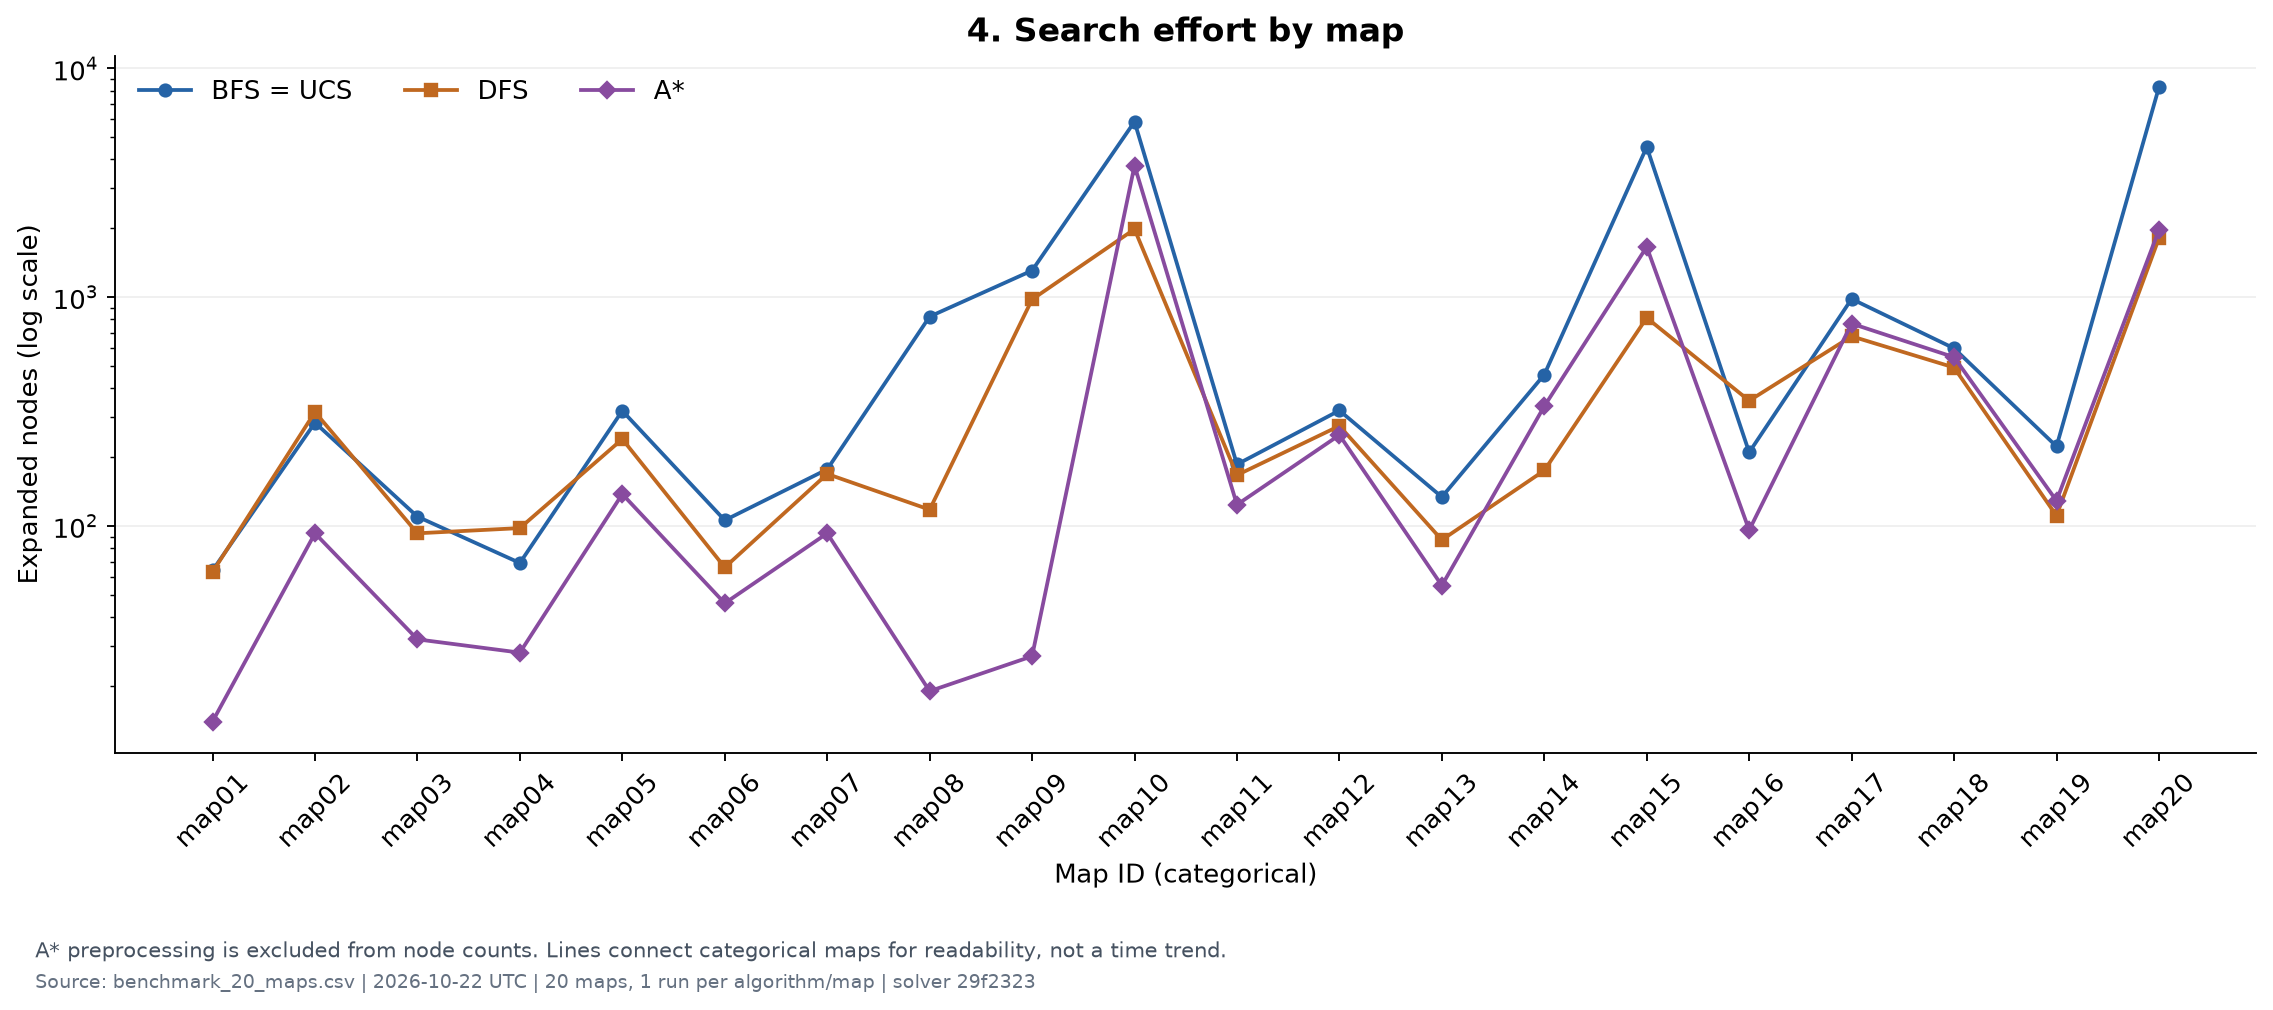
\includegraphics[width=\textwidth]{figures/benchmark_nodes.png}
    \caption{Node mở rộng trên 20 maps. Hai chuỗi BFS và UCS trùng
    nhau trong dữ liệu nên được gộp thành một đường. Nguồn: CSV tại
    commit solver \texttt{29f2323}.}
    \label{fig:benchmark_nodes}
\end{figure}

\begin{figure}[p]
    \centering
    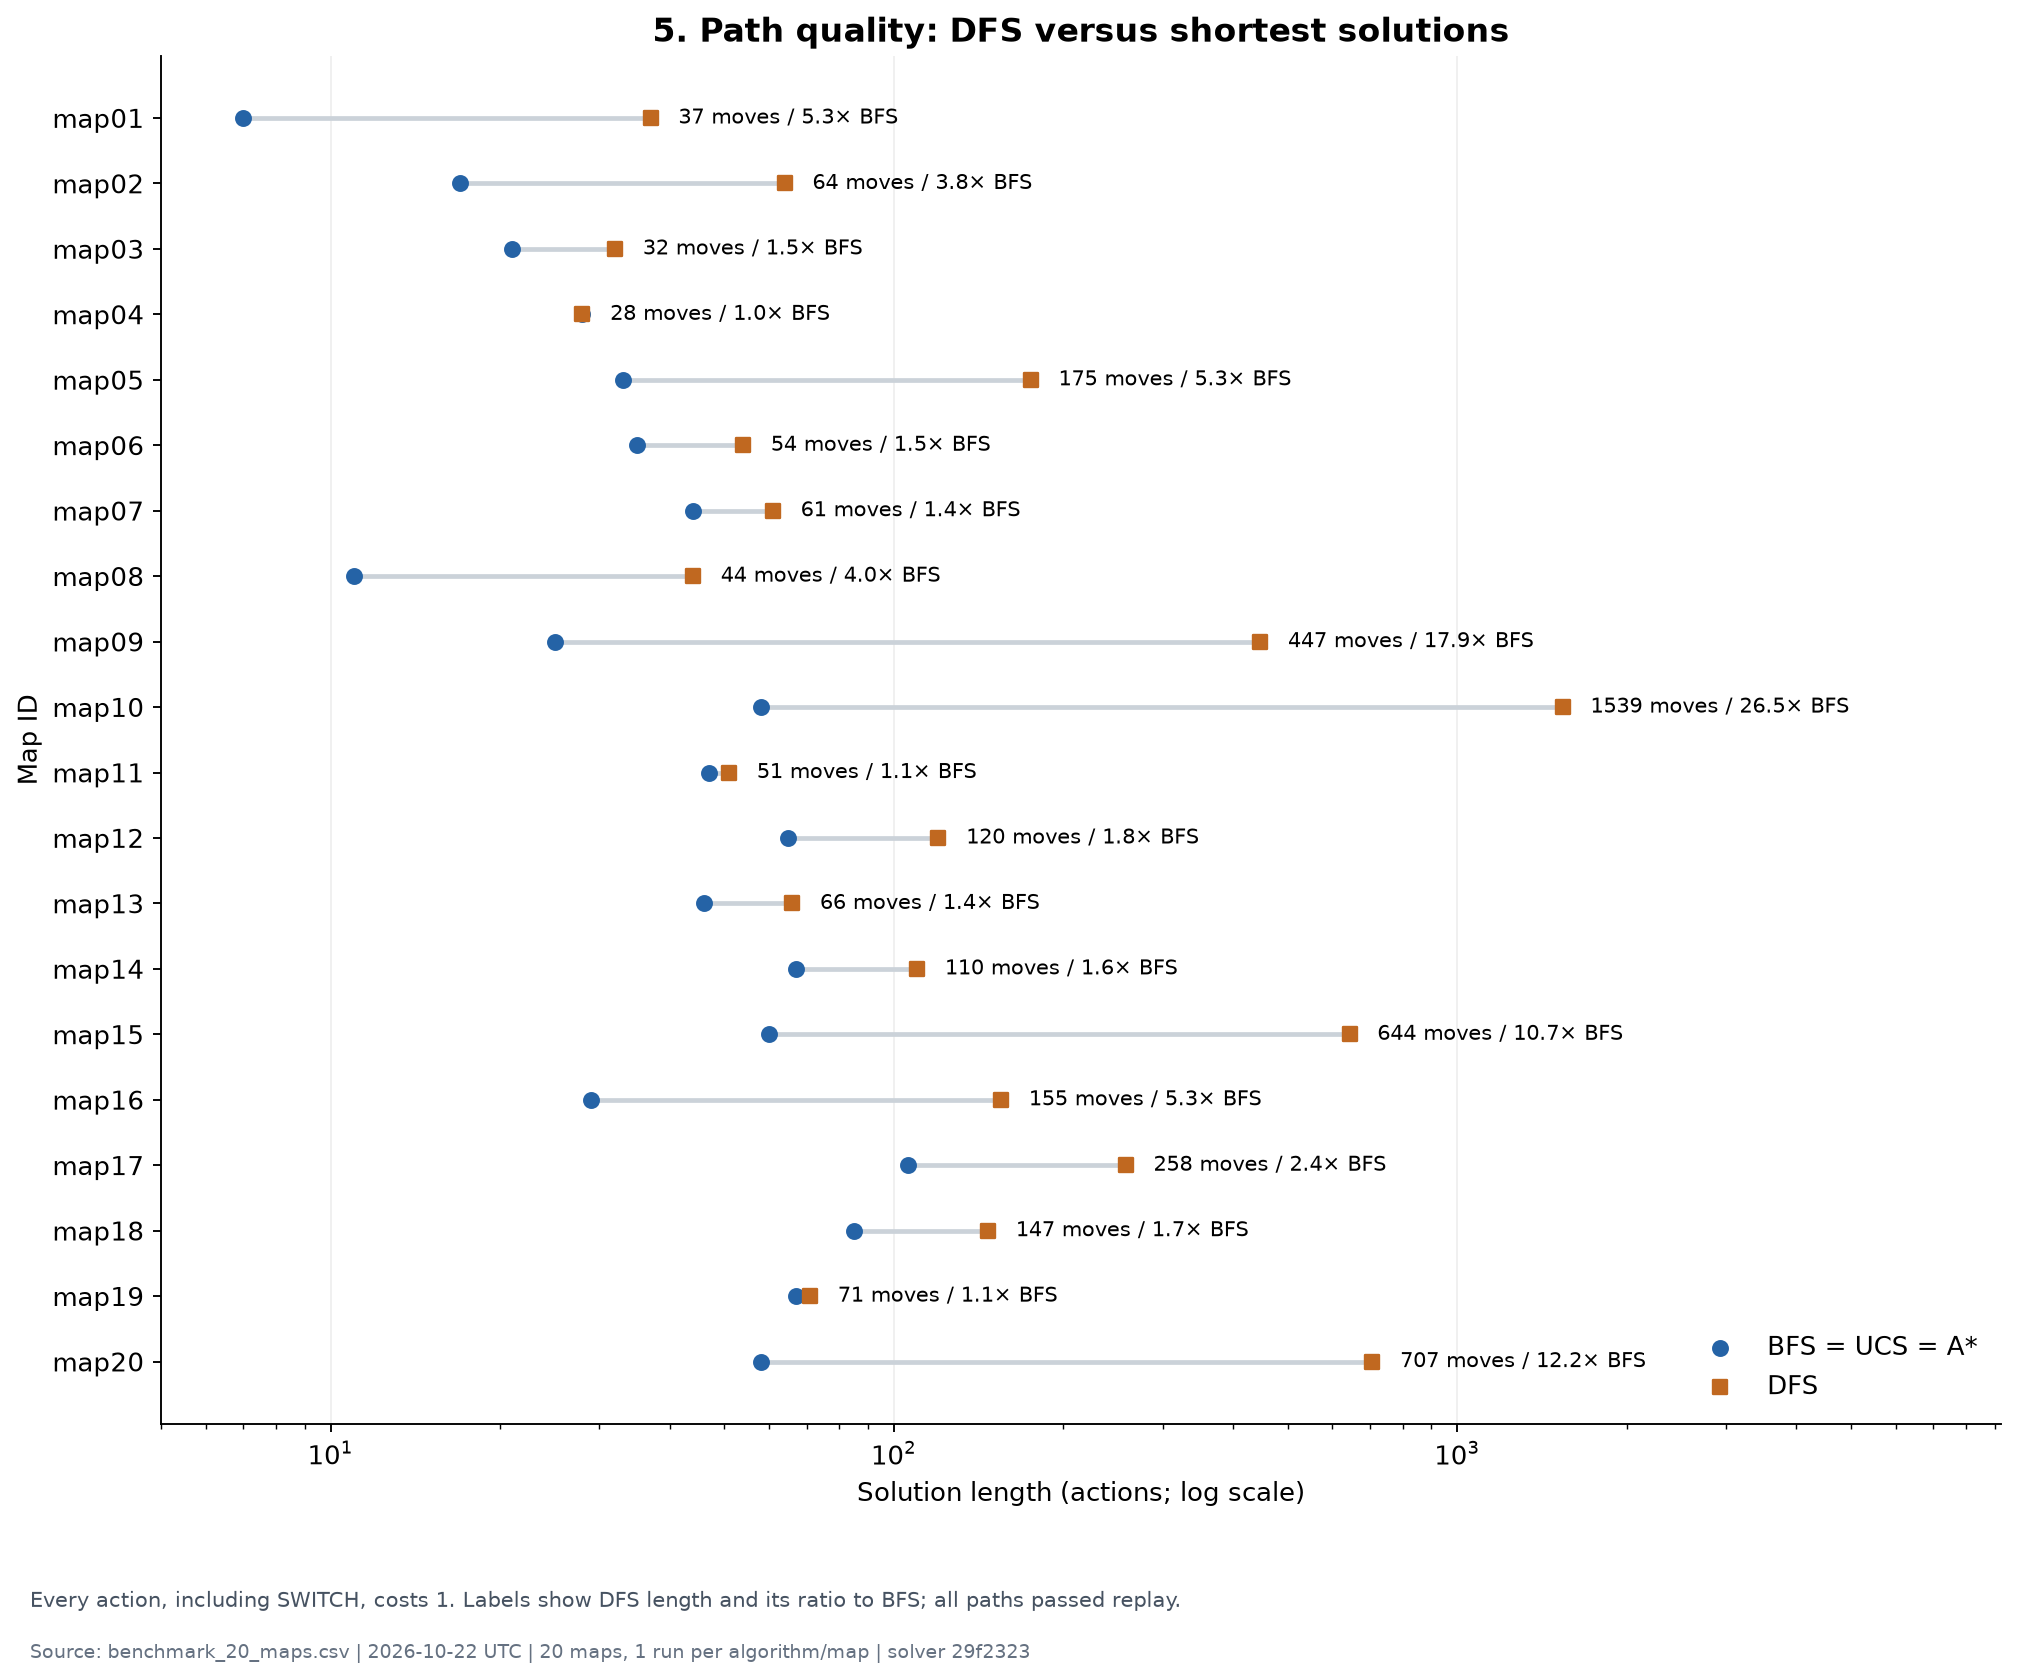
\includegraphics[width=\textwidth,height=0.73\textheight,keepaspectratio]{figures/benchmark_lengths.png}
    \caption{So sánh độ dài lời giải DFS với BFS/UCS/A* trên 20 maps.
    Trục số hành động dùng thang log; hệ số thể hiện số bước DFS chia
    cho số bước BFS trên cùng map.}
    \label{fig:benchmark_lengths}
\end{figure}

\begin{figure}[p]
    \centering
    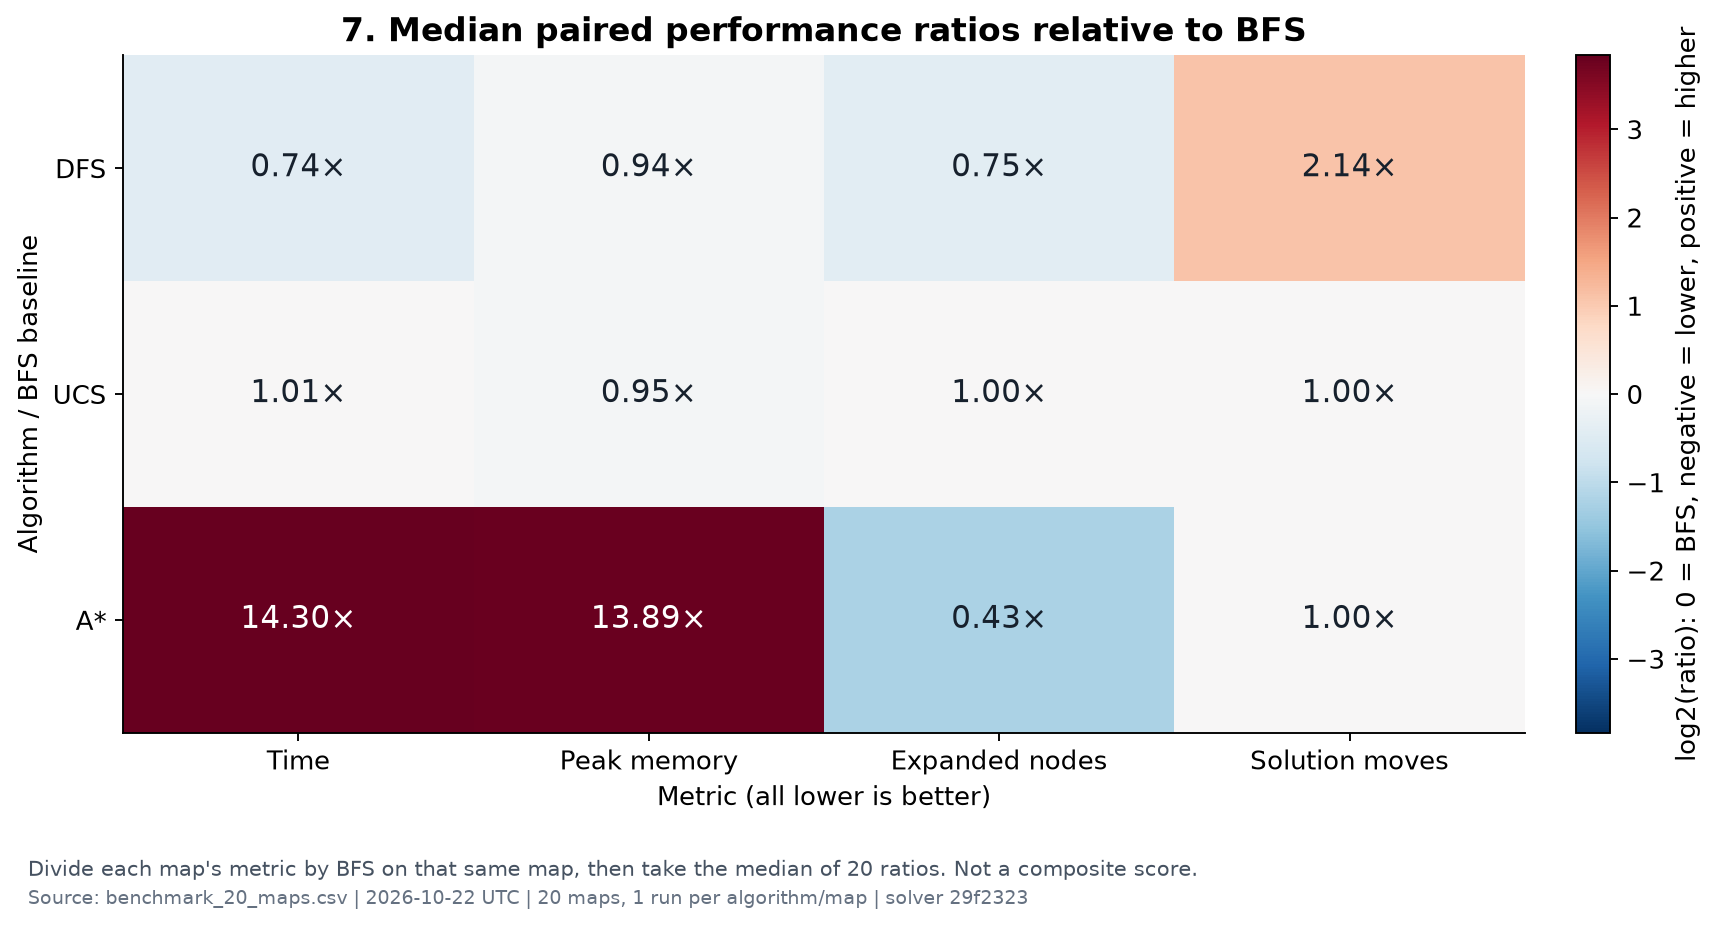
\includegraphics[width=\textwidth]{figures/benchmark_ratios.png}
    \caption{Trung vị tỷ lệ theo từng map so với BFS. Giá trị 1 là
    bằng BFS; thấp hơn 1 là nhỏ hơn ở đại lượng tương ứng. Màu dùng
    thang log cơ số 2 để biểu diễn tỷ lệ.}
    \label{fig:benchmark_ratios}
\end{figure}

\subsection{Hạn chế và hướng mở rộng}

Mỗi cặp map--thuật toán chỉ có một lượt đo nên chưa thể đánh giá độ
ổn định hoặc xây dựng khoảng tin cậy về thời gian. Chênh lệch nhỏ giữa
BFS và UCS không đủ để kết luận ưu thế hiệu năng tổng quát. Boxplot
hiện mô tả sự khác nhau giữa các maps, không mô tả nhiễu qua nhiều
lần chạy cùng đầu vào.

Các bước tiếp theo phù hợp là lặp lại phép đo trên cùng phiên bản
code, lưu số thứ tự trial, thay đổi thứ tự chạy để giảm ảnh hưởng
thứ tự, và tách thời gian dựng heuristic khỏi thời gian tìm kiếm khi
cần phân tích sâu A*. Nếu đo thêm RSS hoặc thay đổi ý nghĩa các cột,
cần bổ sung đại lượng hoặc nâng phiên bản schema thay vì ghi đè ý
nghĩa của số liệu hiện có.
\clearpage

\newpage
\section*{Phụ lục: Sử dụng Trí tuệ Nhân tạo (Generative AI)}
\addcontentsline{toc}{section}{Phụ lục: Sử dụng Trí tuệ Nhân tạo (Generative AI)}

Trong quá trình thực hiện đồ án, nhóm chúng em đã sử dụng các công cụ Trí tuệ nhân tạo tạo sinh (Generative AI) bao gồm ChatGPT, Gemini, Claude và Codex như một trợ lý ảo để tối ưu hóa thời gian làm việc. Cụ thể, AI được ứng dụng trong các khâu:
\begin{itemize}
    \item \textbf{Thiết kế hệ thống:} Gợi ý cách phân rã các lớp (class) Hướng đối tượng cho bản đồ và các loại gạch (Tiles, Bridges).
    \item \textbf{Tìm kiếm giải pháp:} Đề xuất các hàm Heuristic tiềm năng cho thuật toán A* và giải thích các khái niệm học thuật.
    \item \textbf{Sửa lỗi (Debugging):} Hỗ trợ dò tìm lỗi trong giao diện UI và tối ưu hóa cấu trúc dữ liệu.
    \item \textbf{Trình bày văn bản:} Hỗ trợ định dạng cấu trúc báo cáo bằng ngôn ngữ LaTeX.
\end{itemize}

Nhóm cam kết chỉ sử dụng AI ở mức độ tham khảo và hỗ trợ định hướng. Toàn bộ logic cốt lõi của các thuật toán (BFS, DFS, UCS, A*) đều do các thành viên tự cài đặt và tinh chỉnh. Dưới đây là nhật ký các câu lệnh (prompts) chính mà nhóm đã sử dụng:

\renewcommand{\arraystretch}{1.3}
\begin{longtable}{|>{\raggedright\arraybackslash}p{7.5cm}|l|l|}
    \caption{Prompt Logs của nhóm}
    \label{tab:prompt_logs} \\
    \hline
    \textbf{Câu lệnh (Prompt)} & \textbf{Nền tảng} & \textbf{Người sử dụng} \\
    \hline
    \endfirsthead
    
    \multicolumn{3}{c}
    {\tablename\ \thetable\ -- \textit{Tiếp tục từ trang trước}} \\
    \hline
    \textbf{Câu lệnh (Prompt)} & \textbf{Nền tảng} & \textbf{Người sử dụng} \\
    \hline
    \endhead
    
    \hline
    \multicolumn{3}{r}{\textit{Xem tiếp trang sau...}} \\
    \endfoot
    
    \endlastfoot

    Với bài toán Bloxorz Solver, hàm heuristic tôi dùng khoảng cách Manhattan thì có vẻ không hiệu quả. Hãy đề xuất cho tôi cách tiếp cận khác & ChatGPT & Hoàng Minh \\
    \hline
    Bạn xem thuật toán A* hiện tại tôi cài đúng hướng chưa. Cái heuristic còn trường hợp bị chia đôi tôi chưa cài, nên bạn xem tạm thuật toán thôi & Codex & Hoàng Minh \\
    \hline
    Sinh cho tôi 5 testcase từ 20 maps, đảm bảo đủ các trường hợp Bridge, Switch, Teleport,... & Codex & Hoàng Minh \\
    \hline
    Truy cập trang http://www.mlsite.net/bloxorx/, xem 25 maps đầu tiên và tiến hành khởi tạo maps dựa vào những thứ có sẵn trong project này cho tôi & Codex & Hoàng Minh \\
    \hline
    Tạo class Tile, Bridge, FragileTile bằng @dataclass(frozen=True) trong Python. Tách trạng thái đóng/mở cầu ra cho GameState quản lý & Gemini & Phan Nhật Minh \\
    \hline
    Viết class BaseSolver có hàm solve() bọc ngoài để đo time với tracemalloc. Bên trong gọi hàm trừu tượng \_search() để các thuật toán con kế thừa & Gemini & Phan Nhật Minh \\
    \hline
    Cài thuật toán BFS kế thừa BaseSolver. Dùng collections.deque làm hàng đợi và set để lưu state đã duyệt & Gemini & Phan Nhật Minh \\
    \hline
    Hiện tại UI đang bị lỗi khi hiển thị benchmark. Hãy giúp tôi cố định lại khung benchmark khi chạy các thuật toán & Claude & Nguyễn Thành Bảo \\
    \hline
    fix bug đi & Claude & Nguyễn Xuân Lộc \\
    \hline
    Kiểm tra những điểm conflict giữa nhánh hiện tại và main & Claude & Nguyễn Xuân Lộc \\
    \hline
    Khởi tạo thêm 15 map mới dựa trên 20 map hiện tại & Claude & Nguyễn Xuân Lộc \\
    \hline
    Dựa vào code hiện tại, sinh các file test cho tôi, bao gồm: test di chuyển, test map, test logic & Codex & Đỗ Ngọc Hải \\ 
    \hline
    Hãy review thuật toán DFS của tôi, sinh ra các file test và benchmark & Codex & Đỗ Ngọc Hải \\


\end{longtable}
% \section{Kiểm thử và phạm vi đóng góp}

\subsection{Kiểm thử tích hợp}

Các nhóm kiểm thử tập trung vào hành vi có thể quan sát:
\begin{itemize}
    \item UCS: đối chiếu chi phí với BFS, replay hợp lệ, không làm đổi
    trạng thái đầu vào, xử lý chu trình và đường đi có chi phí cải thiện.
    \item Benchmark: lời giải của cả bốn thuật toán, số node ở các
    trường hợp nhỏ, trạng thái đã ở đích/vô nghiệm, giới hạn và dọn bộ đo
    khi lỗi xảy ra.
    \item UI: worker thật dùng \texttt{spawn}, chạy và hủy tìm kiếm,
    replay, đổi khối con, xuất CSV và không làm thay đổi tiến độ chiến
    dịch khi dùng solver.
    \item Visualization: phép tổng hợp và tỷ lệ theo cùng map; phát
    hiện dữ liệu trùng, thiếu, trộn run, sai chi phí hoặc replay không
    hợp lệ; không thay số liệu thiếu bằng 0.
\end{itemize}

Tại merge commit \texttt{8f1f183}, bộ kiểm thử ghi nhận 237 tests đạt.
Sau khi cập nhật \texttt{main} tới \texttt{a89aad2}, bộ kiểm thử hiện có
ghi nhận 228 tests đạt và 8 kiểm tra visualization đạt. Hai con số
thuộc hai phiên bản có tập test khác nhau; bản cập nhật đã bỏ file
test DFS riêng và bổ sung kiểm tra maps mới, nên không diễn giải sự
thay đổi số lượng thành mức tăng hoặc giảm chất lượng phần mềm.
Các lệnh kiểm tra tương ứng từ thư mục gốc:

\begin{lstlisting}[language=bash]
python -m pytest -q
python -m unittest visualization.checks -v
\end{lstlisting}

Các kết quả trên xác nhận những trường hợp được kiểm thử, không thay
thế chứng minh tính đúng của thuật toán hoặc bảo đảm không còn lỗi
trên mọi đầu vào. Phép đo hiệu năng trong Mục~\ref{sec:benchmark}
vẫn dùng CSV lịch sử, không lấy thời gian chạy test làm benchmark.

\subsection{Phạm vi phần việc được trình bày}

Phần đóng góp của Nguyễn Thành Bảo được mô tả trong các mục trên gồm:
cài đặt UCS; tích hợp chế độ chạy thuật toán và replay vào UI; chuẩn
hóa phép đo benchmark; xây dựng CSV 20 maps và schema; tạo notebook
với bảy biểu đồ; xử lý tương thích và kiểm thử khi merge với code nhóm.

Bộ luật chơi, giao diện nền, BFS, DFS và heuristic A* là các thành
phần chung của nhóm được sử dụng hoặc điều chỉnh để tích hợp. Bộ 15
maps mới trên \texttt{main} là phần bổ sung của nhóm, không được nhận
là phần tự xây dựng trong phạm vi công việc này. Mức độ hoàn thành
và phân công cuối cùng cần được các thành viên thống nhất.

Trong quá trình thực hiện có sử dụng trợ lý AI Codex để hỗ trợ soạn
và chỉnh sửa code, tạo kiểm thử, xử lý tích hợp Git và tổng hợp nội
dung báo cáo. Bản thảo này được đối chiếu với mã nguồn, CSV và kết
quả kiểm thử trong repository; người thực hiện cần rà soát nội dung
và tuân theo quy định khai báo hỗ trợ AI của môn học trước khi nộp.
 Mục này cần xem lại
% ==============================================================================
% TÀI LIỆU THAM KHẢO (BIBLIOGRAPHY)
% ==============================================================================
\newpage
\nocite{*}
\bibliographystyle{plain}
\bibliography{references}

\end{document}
